% Official PVLDB Volume 20 / VLDB 2027 template
% (https://github.com/vldbproceedings/VLDB-Template, acmart.cls v2.19 2026/06/27).
% Regular research paper: at most 12 pages excluding references
% (https://www.vldb.org/2027/submission-guidelines.html).
\documentclass[sigconf, nonacm]{acmart}

%%% do not modify the following VLDB block %%
%%% VLDB block start %%%
\usepackage{pvldb}% VLDB/PVLDB formatting overrides, see pvldb.sty for details.
                      % Do not remove -- required for consistent proceedings
                      % formatting across all VLDB submissions.
%%% VLDB block end %%%

%% The following must be set for each paper (values below are placeholders).
\renewcommand\vldbdoi{XX.XX/XXX.XX}
\renewcommand\vldbpages{XXX-XXX}
\renewcommand\vldbavailabilityurl{https://github.com/wanghongsheng01/ScopeCache}

\usepackage[T1]{fontenc}  % for \DJ and other accented names in the references
\usepackage{array}
\usepackage{multirow}
\usepackage{xcolor}
% Avoid clash with acmart's algorithm environment
\let\algorithm\relax
\let\endalgorithm\relax
\usepackage[ruled,linesnumbered,vlined]{algorithm2e}
% acmart defines theorem et al. at \begin{document}
\emergencystretch=1em  % allow slightly looser line breaks instead of overfull boxes

\AtBeginDocument{%
  \newtheorem{assumption}[theorem]{Assumption}%
  \hypersetup{hidelinks}%
}
\newcommand{\M}[1]{\textsf{#1}}
\newcommand{\scope}{\mathit{scope}}
\newcommand{\Takeaway}[1]{\smallskip\noindent\fbox{\parbox{0.97\columnwidth}{\small\textbf{Takeaway.} #1}}\smallskip}
\SetKwComment{tcp}{// }{}
\SetAlFnt{\small}
% generated by tools/make_numbers.py -- do not edit
\newcommand{\abBest}{3}
\newcommand{\abCols}{5}
\newcommand{\abGmAtoms}{1.00}
\newcommand{\abGmNolift}{1.02}
\newcommand{\abGmOnline}{1.55}
\newcommand{\abGmPSPlus}{2.69}
\newcommand{\abGmSnap}{1.63}
\newcommand{\abSecond}{1}
\newcommand{\agBestCells}{8}
\newcommand{\agCells}{8}
\newcommand{\agSecondCells}{0}
\newcommand{\agentCallsPerEpHi}{2.8}
\newcommand{\agentCallsPerEpLo}{1.4}
\newcommand{\agentCost}{3.17}
\newcommand{\agentPSHi}{50}
\newcommand{\agentPSLo}{19}
\newcommand{\agentPSMeanHi}{35}
\newcommand{\agentPSMeanLo}{29}
\newcommand{\agentPSVSentence}{Against \M{PerScope+V}, which has the same pinned views, ScopeCache needs 29--74\% fewer executions on TPC-H and TPC-DS and as many on BIRD and ENT, where pinned views answer 96--98\% of data calls.}
\newcommand{\agentPSVneg}{0}
\newcommand{\agentRedOnlinePSHi}{98}
\newcommand{\agentRedOnlinePSLo}{33}
\newcommand{\agentRedPSVHi}{85}
\newcommand{\agentRedPSVLo}{0}
\newcommand{\agentRedPSVMeanHi}{74}
\newcommand{\agentRedPSVMeanLo}{0}
\newcommand{\agentRedPSVMed}{0}
\newcommand{\agentRedVRmed}{20}
\newcommand{\agentScHitHi}{99}
\newcommand{\agentScHitLo}{95}
\newcommand{\agentSemHitHi}{98}
\newcommand{\agentSemHitLo}{89}
\newcommand{\agentSemOverHi}{86}
\newcommand{\agentSemOverLo}{60}
\newcommand{\agentVRHitHi}{98}
\newcommand{\agentVRHitLo}{75}
\newcommand{\agentXscopeEnt}{38}
\newcommand{\agentXscopeEntD}{38.1}
\newcommand{\agentXscopeHi}{98}
\newcommand{\agentXscopeLo}{36}
\newcommand{\agentXscopeMeanHi}{93}
\newcommand{\agentXscopeMeanLo}{38}
\newcommand{\artifactURL}{https://github.com/wanghongsheng01/ScopeCache}
\newcommand{\atomsDeltaHi}{+16}
\newcommand{\atomsDeltaLo}{$-$8}
\newcommand{\atomsEntExecDiff}{2}
\newcommand{\atomsEntFbRed}{8}
\newcommand{\atomsMeanSave}{3}
\newcommand{\atomsMeanWorse}{5}
\newcommand{\bdOtherHi}{20}
\newcommand{\bdOtherLo}{0}
\newcommand{\bdSameHi}{2}
\newcommand{\bdSameLo}{0}
\newcommand{\bdSelfHi}{9}
\newcommand{\bdSelfLo}{1}
\newcommand{\bdSelfSameHi}{9}
\newcommand{\bdSelfSameLo}{1}
\newcommand{\bdViewHi}{92}
\newcommand{\bdViewLo}{60}
\newcommand{\bdXHi}{20}
\newcommand{\bdXLo}{0}
\newcommand{\callsPerQHi}{2.5}
\newcommand{\callsPerQLo}{1.7}
\newcommand{\deriveMsHi}{18}
\newcommand{\deriveMsLo}{10}
\newcommand{\domBest}{4}
\newcommand{\domPSHitHi}{28}
\newcommand{\domPSHitLo}{25}
\newcommand{\domPoints}{4}
\newcommand{\domRedPSPlusHi}{64}
\newcommand{\domRedPSPlusLo}{36}
\newcommand{\domRedPSVHi}{19}
\newcommand{\domRedPSVLo}{0}
\newcommand{\domRedVRHi}{41}
\newcommand{\domRedVRLo}{13}
\newcommand{\domScHitHi}{94}
\newcommand{\domScHitLo}{86}
\newcommand{\domTies}{1}
\newcommand{\driftRedHi}{27}
\newcommand{\driftRedLo}{12}
\newcommand{\entBigRedPSPlus}{81}
\newcommand{\entBigXscope}{87}
\newcommand{\evBest}{16}
\newcommand{\evHitDropMax}{0.8}
\newcommand{\evPSHi}{1{,}813}
\newcommand{\evPSLo}{1{,}491}
\newcommand{\evPSVTieSetups}{BIRD and ENT}
\newcommand{\evPoints}{20}
\newcommand{\evSynfgHitSixteen}{67.3}
\newcommand{\evSynfgHitZero}{67.5}
\newcommand{\fallbackHi}{11}
\newcommand{\fallbackLo}{6}
\newcommand{\intlCalls}{2{,}605}
\newcommand{\intlMTokens}{4.9}
\newcommand{\lookupPninetyFiveHi}{63}
\newcommand{\lookupPninetyFiveLo}{30}
\newcommand{\mainCells}{10}
\newcommand{\nAgentCalls}{13{,}013}
\newcommand{\nAgentDataCalls}{9{,}164}
\newcommand{\nAgentTraces}{32}
\newcommand{\nMainDataCalls}{31{,}273}
\newcommand{\nMainRuns}{15}
\newcommand{\nModelsWord}{five}
\newcommand{\nPSVneg}{3}
\newcommand{\nPSVruns}{15}
\newcommand{\nRedVRpos}{15}
\newcommand{\nRedVRruns}{15}
\newcommand{\nSafeCachesWord}{twelve}
\newcommand{\nSafeDataCalls}{375{,}276}
\newcommand{\nScopesHi}{132}
\newcommand{\nScopesLo}{85}
\newcommand{\nVRAbestNeg}{0}
\newcommand{\nVendorsWord}{five}
\newcommand{\noliftAbsMax}{4}
\newcommand{\noliftExecMore}{4}
\newcommand{\noliftExecRedVR}{17}
\newcommand{\noliftHi}{+9}
\newcommand{\noliftLo}{$-$2}
\newcommand{\noliftRowsRedVR}{16}
\newcommand{\onlineFactorEnt}{4.3}
\newcommand{\onlineFactorHi}{4.30}
\newcommand{\onlineFactorLo}{0.96}
\newcommand{\onlineNoliftEnt}{1.00}
\newcommand{\onlineNoliftHi}{1.85}
\newcommand{\onlineNoliftLo}{1.28}
\newcommand{\onlineNoliftSaveHi}{46}
\newcommand{\onlineNoliftSaveLo}{22}
\newcommand{\oracleAgree}{1{,}473}
\newcommand{\oracleChecked}{1{,}473}
\newcommand{\padFastHi}{9}
\newcommand{\padFastLo}{1}
\newcommand{\partHitHi}{27}
\newcommand{\partHitLo}{14}
\newcommand{\ppHitHi}{75}
\newcommand{\ppHitLo}{52}
\newcommand{\psvSmallHi}{4}
\newcommand{\psvTpchHi}{15}
\newcommand{\psvTpchLo}{5}
\newcommand{\psvZeroSetups}{BIRD and ENT}
\newcommand{\redNCHi}{93}
\newcommand{\redNCLo}{69}
\newcommand{\redPSHi}{98}
\newcommand{\redPSLo}{93}
\newcommand{\redPSPlusHi}{54}
\newcommand{\redPSPlusLo}{23}
\newcommand{\redPSPlusMed}{51}
\newcommand{\redPSVHi}{15}
\newcommand{\redPSVLo}{-7}
\newcommand{\redPSVMed}{0}
\newcommand{\redPSmainHi}{91}
\newcommand{\redPSmainLo}{57}
\newcommand{\redVRAHi}{36}
\newcommand{\redVRALo}{9}
\newcommand{\redVRAbestHi}{32}
\newcommand{\redVRAbestLo}{9}
\newcommand{\redVRHi}{37}
\newcommand{\redVRLo}{9}
\newcommand{\redVRMed}{21}
\newcommand{\redVRtpch}{31}
\newcommand{\rerunDiff}{8}
\newcommand{\rerunN}{12}
\newcommand{\rerunSame}{2}
\newcommand{\rivalBestN}{6}
\newcommand{\rivalName}{\M{PerScope+V}}
\newcommand{\rivalSecondN}{4}
\newcommand{\rivalStanding}{best (tied) in 6 and second in 4 cells}
\newcommand{\rowsPerExecSCHi}{2.0}
\newcommand{\rowsPerExecSCLo}{0.8}
\newcommand{\rowsRedNCHi}{95}
\newcommand{\rowsRedNCLo}{60}
\newcommand{\rowsRedPSHi}{93}
\newcommand{\rowsRedPSLo}{46}
\newcommand{\rowsRedPSPlusHi}{85}
\newcommand{\rowsRedPSPlusLo}{20}
\newcommand{\rowsRedPSVHi}{13}
\newcommand{\rowsRedPSVLo}{-9}
\newcommand{\rowsSentence}{Counting fact-table rows instead of executions, ScopeCache scans 46--93\% fewer rows than \M{PerScope}, its online path 20--85\% fewer than \M{PerScope+}, and the full system 6--14\% fewer than \M{ViewRewrite} on TPC-H, BIRD, ENT, and SYN-FG. On TPC-DS, a ScopeCache execution scans 1.4$\times$ the rows of a \M{ViewRewrite} execution, because a lifted execution covers a wider window than the call that triggers it, whereas a miss of \M{ViewRewrite} scans only the requested window; ScopeCache therefore scans 14\% more rows there while needing fewer executions.}
\newcommand{\rowsUnfMore}{14}
\newcommand{\rowsUnfSetup}{TPC-DS}
\newcommand{\scBestCells}{8}
\newcommand{\scEntExecSd}{20}
\newcommand{\scHitHi}{93.3}
\newcommand{\scHitLo}{69.3}
\newcommand{\scSecondCells}{2}
\newcommand{\scaleDataCalls}{2{,}175}
\newcommand{\scaleRedPS}{81}
\newcommand{\scaleRedPSPlus}{53}
\newcommand{\scaleRedPSV}{7}
\newcommand{\scaleRedVR}{28}
\newcommand{\scaleRedVROne}{30}
\newcommand{\scaleScHit}{85}
\newcommand{\semOverHi}{33}
\newcommand{\semOverLo}{12}
\newcommand{\sensOneCalls}{919}
\newcommand{\sensOneEnt}{21}
\newcommand{\sensOneHi}{77}
\newcommand{\sensOneLo}{14}
\newcommand{\sensOneTpch}{59}
\newcommand{\sensTwoHi}{91}
\newcommand{\sensTwoLo}{26}
\newcommand{\smallRedHi}{47}
\newcommand{\smallRedLo}{21}
\newcommand{\snapFactorHi}{4.18}
\newcommand{\snapFactorLo}{1.01}
\newcommand{\snapFactorSixteen}{5.3}
\newcommand{\synfgEvictedHi}{640}
\newcommand{\synfgEvictedLo}{545}
\newcommand{\synfgGroups}{300}
\newcommand{\synfgMax}{40}
\newcommand{\synfgMean}{2.3}
\newcommand{\synfgMedian}{1}
\newcommand{\synfgMorePSVHi}{6.6}
\newcommand{\synfgMorePSVLo}{1.4}
\newcommand{\synfgOnlineExecHi}{617}
\newcommand{\synfgOnlineExecLo}{586}
\newcommand{\synfgOnlineVsSCHi}{3.9}
\newcommand{\synfgOnlineVsSCLo}{3.7}
\newcommand{\synfgPSHitHi}{28.6}
\newcommand{\synfgPSHitLo}{26.5}
\newcommand{\synfgRedPSHi}{59.5}
\newcommand{\synfgRedPSLo}{56.8}
\newcommand{\synfgRedPSVHi}{-1.4}
\newcommand{\synfgRedPSVLo}{-6.6}
\newcommand{\synfgRedVRHi}{24.6}
\newcommand{\synfgRedVRLo}{22.5}
\newcommand{\synfgRows}{6.0}
\newcommand{\synfgScExecHi}{641}
\newcommand{\synfgScExecLo}{610}
\newcommand{\synfgScHitHi}{70.6}
\newcommand{\synfgScHitLo}{69.3}
\newcommand{\synfgScopes}{300}
\newcommand{\synfgSensitivePct}{25}
\newcommand{\synfgSharedGroups}{60}
\newcommand{\synfgShops}{300}
\newcommand{\synfgSingletons}{240}
\newcommand{\synfgUsers}{700}
\newcommand{\ttlReplayCalls}{419}
\newcommand{\ttlReplayWrong}{136}
\newcommand{\viewMaintHi}{14}
\newcommand{\viewMaintLo}{0}
\newcommand{\viewSelSecMax}{6}
\newcommand{\vrAdaptRebuilds}{3}
\newcommand{\vrHitBird}{92}
\newcommand{\vrHitEnt}{90}
\newcommand{\vrMaintViews}{0--14}
\newcommand{\vrSecondCells}{4}
\newcommand{\vraChangedSetups}{TPC-H, BIRD, and SYN-FG}
\newcommand{\vraHitGainMax}{1.9}

% --- frozen SC-adaptP headline (v7fresh, seeds 3-5); do not regenerate from v5 ---
\newcommand{\freshDataCalls}{31{,}964}
\newcommand{\freshOursTot}{4{,}512}
\newcommand{\freshPSVTot}{4{,}804}
\newcommand{\freshHybTot}{4{,}813}
\newcommand{\freshRedTot}{6.1}
\newcommand{\psvW}{10}
\newcommand{\psvT}{5}
\newcommand{\psvL}{0}
\newcommand{\hybWTL}{6--6--3}
\newcommand{\scVsHybWTL}{7--7--1}
\newcommand{\unpinMinFrozen}{40}
\newcommand{\freshHitLo}{68.9}
\newcommand{\freshHitHi}{93.0}
\newcommand{\evSynfgRedLo}{9.2}
\newcommand{\evSynfgRedHi}{14.3}

% --- analysis of frozen v7fresh (not a new eval); bootstrap seed 20261112, B=10000 ---
\newcommand{\freshDeltaPsv}{292}
\newcommand{\freshDeltaHyb}{301}
\newcommand{\freshCIpsvLo}{$-$516}
\newcommand{\freshCIpsvHi}{$-$101}
\newcommand{\freshCIhybLo}{$-$575}
\newcommand{\freshCIhybHi}{$-$61}
\newcommand{\freshPpsv}{<0.001}
\newcommand{\freshPhyb}{0.010}
\newcommand{\lossUnpinRows}{676{,}933}
\newcommand{\lossHitViewOurs}{1{,}430}
\newcommand{\lossHitViewHyb}{1{,}662}
\newcommand{\lossValCalls}{148}
\newcommand{\lossGhost}{42}
\newcommand{\lossUnpins}{4}
\newcommand{\lossExtraExec}{20}
\newcommand{\adaptSelSecLo}{10}
\newcommand{\adaptSelSecHi}{40}
\newcommand{\adaptSelSecMed}{20}
\newcommand{\ovhPfiftyOursMed}{5.4}
\newcommand{\ovhPfiftyHybMed}{5.2}
\newcommand{\ovhPfiftyOursLo}{2.7}
\newcommand{\ovhPfiftyOursHi}{7.2}
\newcommand{\bootSeed}{20261112}
\newcommand{\bootB}{10{,}000}

% --- pre-registered v8 robustness (seeds 6-10); does not replace the v7fresh headline ---
\newcommand{\robOurs}{7{,}336}
\newcommand{\robPsv}{7{,}754}
\newcommand{\robHyb}{7{,}651}
\newcommand{\robAtoms}{7{,}623}
\newcommand{\robWTLPsv}{15--9--1}
\newcommand{\robWTLHyb}{5--16--4}
\newcommand{\robRedPsv}{5.4}
\newcommand{\robCIpsvLo}{$-$710}
\newcommand{\robCIpsvHi}{$-$171}
\newcommand{\robCIhybLo}{$-$714}
\newcommand{\robCIhybHi}{15}
\newcommand{\robCIatLo}{$-$623}
\newcommand{\robCIatHi}{8}
\newcommand{\robLossExec}{280}
\newcommand{\robLossPsv}{264}
\newcommand{\robLossHyb}{247}
\newcommand{\shiftOurs}{9{,}326}
\newcommand{\shiftPsv}{10{,}345}
\newcommand{\shiftHyb}{10{,}179}
\newcommand{\shiftAtoms}{10{,}082}
\newcommand{\shiftWTLPsv}{15--10--0}
\newcommand{\shiftWTLHyb}{10--15--0}
\newcommand{\shiftRedPsv}{9.9}
\newcommand{\shiftRedHyb}{8.4}
\newcommand{\shiftCIpsvLo}{$-$1{,}576}
\newcommand{\shiftCIpsvHi}{$-$509}
\newcommand{\shiftCIhybLo}{$-$1{,}382}
\newcommand{\shiftCIhybHi}{$-$385}
\newcommand{\shiftCIatLo}{$-$1{,}216}
\newcommand{\shiftCIatHi}{$-$356}
\newcommand{\shiftTpchTenOurs}{417}
\newcommand{\shiftTpchTenPsv}{509}
\newcommand{\shiftTpchTenHyb}{453}


\begin{document}

\title[ScopeCache: Safe Reuse of Query Results Across Permission Scopes]{ScopeCache: Safe Reuse of Query Results Across Permission Scopes for Multi-Principal Data Agents}

%% Author list frozen.
\author{Hongsheng Wang}
\authornote{Corresponding author.}
\orcid{0009-0009-8214-5150}
\affiliation{%
  \institution{Zhejiang University}
  \department{College of Computer Science and Technology}
  \city{Hangzhou}
  \state{310058}
  \country{China}
}
\affiliation{%
  \institution{Loctek Ergonomic Technology Corp.}
  \department{Artificial Intelligence Department}
  \city{Ningbo}
  \state{315100}
  \country{China}
}
\email{wanghongsheng@zju.edu.cn}

\author{Dazhen Deng}
\authornote{Corresponding author.}
\orcid{0000-0002-9057-8353}
\affiliation{%
  \institution{Zhejiang University}
  \department{School of Software Technology}
  \city{Ningbo}
  \state{315048}
  \country{China}
}
\email{dengdazhen@zju.edu.cn}

\renewcommand{\shortauthors}{Wang and Deng}

\begin{abstract}
LLM data agents query governed warehouses through metric tools for many employees, each restricted by row- and column-level permissions that change while the agents run, over a semantic layer whose definitions are republished. Existing result caches key entries on the requester or its scope, which confines reuse to principals with identical permissions, or on the query intent alone, which returns other principals' data. We present ScopeCache, a result cache that shares work across principals with different scopes and never returns data outside the requester's view. It stores principal-independent partial aggregates grouped by the policy attributes, applies the requester's current scope and the current metric definitions at lookup time, and lifts predicates on a miss so that one execution serves many principals. We prove that every answer equals a fresh execution under the current policy and semantic layer and depends only on rows in the requester's scope, that permission changes need no invalidation, and that a republish invalidates only the changed measures. On five setups, including a fine-grained synthetic shop policy (SYN-FG) with \synfgUsers{} principals and \synfgScopes{} scopes, and on \nAgentCalls{} metric calls of \nModelsWord{} LLM agents from \nVendorsWord{} vendors, including GPT-6 and Claude Opus~5.5, over the four public and enterprise-synthetic setups, ScopeCache returned no wrong answer, and its online path served \agentXscopeMeanLo--\agentXscopeMeanHi\% of agent data calls (setup means) from entries created under another scope. On fifteen runs whose seeds were held out from design and from the choice of the unpinning threshold, with \freshDataCalls{} differentially tested data calls per cache, it matches or beats the strongest baseline---the same cache partitioned by scope, with the same pinned views---in every run: \psvW{} wins, \psvT{} ties, \psvL{} losses, and \freshRedTot\% fewer warehouse executions in total. Code and traces are released.
\end{abstract}

\maketitle

%%% do not modify the following VLDB block %%
%%% VLDB block start %%%
\vldbtopmatter
%%% VLDB block end %%%

\section{Introduction}
\label{sec:intro}

Enterprises increasingly expose their warehouses to LLM agents through governed tools: a semantic layer compiles a request for metrics, dimensions, filters, and a time range into SQL over a fact table, and a policy engine conjoins the requester's row predicate and rejects hidden columns~\cite{mcpgw26,authzarch26}. Agents generate a heavy and repetitive workload: they explore speculatively, break a metric down, drill into a value, switch metrics, and retry~\cite{agentfirst25,wadlom26}, and many employees' agents ask the same business questions. In the platform that motivated this work, every warehouse call costs a connection, a semantic-snapshot fetch, and the query itself, about half a second at the median, and the platform caches neither tool results nor permission decisions, so that a revoked grant takes effect at the next call. Result reuse is the textbook remedy~\cite{hru96,goldstein01,ivanova09,dursun17}, yet it has been switched off for a structural reason. A warehouse that answers ad-hoc metric questions for many employees---ask-data, as opposed to a closed set of applications---must enforce row- and column-level permissions in its last pre-aggregation layers (the summary and application-data marts), not only in the client application; those layers therefore cannot be dropped the way a warehouse that serves only packaged applications might. Two principals asking the same question are entitled to different answers, and a permission-scoped result cache is the systems counterpart of that constraint: it shares work across scopes without handing authorization to the application and without retaining a large family of pre-declared, permission-specific aggregates.

Existing caches resolve this conflict in one of two ways (Table~\ref{tab:gap}). \emph{Partitioned} caches key an entry on the requester, its role, its scope, or the rewritten statement that already contains its row predicate; Snowflake's result cache and fine-grained-access-control rewriting work this way~\cite{snowflake16,stonebraker74,rizvi04}. They are safe but only principals with identical permissions share entries. \emph{Shared} caches key an entry on the request or its intent, as semantic OLAP caches~\cite{bindschaedler26}, LLM semantic caches~\cite{gptcache23,vcache25}, and agent tool caches do; they reuse across principals but return results computed for someone else. Materialized views with a row predicate applied at query time (VPD over views) avoid both problems when the workload is known in advance~\cite{hru96,chaudhuri07}, but they are chosen offline and recomputed whenever a metric definition changes. In Table~\ref{tab:gap}, a cache is \emph{sound} if every answer equals a fresh execution under the requester's policy, and \emph{online} if it needs no training workload.

\begin{table}[t]
\centering
\caption{Only ScopeCache is sound, shares entries across scopes, works online, and applies permission events at the next call.}
\label{tab:gap}
\footnotesize
\setlength{\tabcolsep}{3pt}
\begin{tabular}{@{}lcccc@{}}
\toprule
Cache & Sound & Cross-scope & Online & Events\\
\midrule
SQL result cache & \checkmark & -- & \checkmark & \checkmark\\
Per-user/scope cache & \checkmark & -- & \checkmark & \checkmark\\
Intent-keyed cache & -- & \checkmark & \checkmark & --\\
Expiring shared cache & -- & \checkmark & \checkmark & --\\
Views + row filter & \checkmark & \checkmark & -- & \checkmark\\
\textbf{ScopeCache} & \checkmark & \checkmark & \checkmark & \checkmark\\
\bottomrule
\end{tabular}
\end{table}

\begin{figure}[t]
\centering
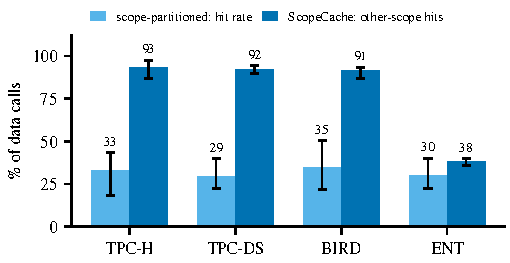
\includegraphics[width=\columnwidth]{fig1_agent.pdf}
\caption{ScopeCache answers \agentXscopeMeanLo--\agentXscopeMeanHi\% of real agents' data calls from entries created under another scope, against \agentPSMeanLo--\agentPSMeanHi\% for a scope-partitioned cache. \nAgentTraces{} real LLM-agent traces; bars: mean, whiskers: range over the traces of a setup. Dark: hits of ScopeCache without pinned views on entries created under a different scope; every hit equals a fresh execution under the requester's policy.}
\label{fig:agent}
\Description{Bar chart of cross-scope hit rates of ScopeCache versus a scope-partitioned cache on real LLM-agent traces, showing the mean and range over the traces of each setup.}
\end{figure}

Partitioning shares little in practice because scopes are fine-grained: under a synthetic shop policy that we call SYN-FG, \synfgUsers{} principals hold \synfgScopes{} distinct shop scopes, and the median scope belongs to a single principal (\synfgMean{} principals per scope on average). Fig.~\ref{fig:agent} measures what partitioning gives up on real agent workloads. We recorded \nModelsWord{} LLM agents (DeepSeek, GLM, Kimi, GPT-6, and Claude) answering business questions for principals with different row scopes over four setups. Averaged per setup, a scope-partitioned cache answers \agentPSMeanLo--\agentPSMeanHi\% of their data calls, whereas \agentXscopeMeanLo--\agentXscopeMeanHi\% of the calls can be derived, exactly and within the requester's view, from aggregates computed for a principal with a \emph{different} scope. The opportunity comes from two sources: different principals ask overlapping questions, and the questions of one agent roll up from, filter, or sub-range the questions of another.

Exploiting this opportunity safely raises three challenges.
\textbf{C1 (Soundness and non-interference).} An answer derived from another principal's work must equal a fresh execution under the requester's row predicate and column grants, and must not depend on rows the requester may not see.
\textbf{C2 (Dynamics).} Memberships, grants, and column permissions change, and the change must take effect at the next call; metric formulas, measure definitions, and dimension mappings are republished, and flushing the cache on every republish wastes the reuse.
\textbf{C3 (Efficiency).} Sharing across scopes must pay for its larger entries within a storage budget, both for an unknown online workload and when a training workload is available.

\textbf{Approach.} ScopeCache stores \emph{principal-independent} partial aggregates. Each entry is computed once, without any row predicate, grouped by the requested dimensions and by all policy attributes, so that every cell lies entirely inside or entirely outside any principal's scope. To address C1, a lookup evaluates the requester's current scope and column grants, keeps only the cells inside the scope, and combines distributive aggregates; non-decomposable aggregates take a scope-keyed fallback path. To address C2, entries contain no principal and no metric formula: permission events require no invalidation, formulas are applied at lookup time, and a republish invalidates only the measure columns whose definition changed. To address C3, a miss lifts filters into the grouping and widens the time window when the result fits an admission bound, computes all measures of the fact table together, and combines online entries with pinned views selected under a budget with a constant-factor guarantee. When a training prefix is available, a holdout over that prefix selects among a small portfolio of view and budget configurations, and a ghost directory unpins views only after an evidence threshold that was frozen before the headline evaluation.

\textbf{Contributions.}
\begin{itemize}
\item We formalize permission- and version-safe result reuse for multi-principal metric workloads, with soundness, non-interference, and freshness under permission and semantic-layer events (Section~\ref{sec:problem}).
\item We design ScopeCache and prove that its answers are sound and non-interfering (Theorem~\ref{thm:sound}), that permission events need no invalidation (Theorem~\ref{thm:events}), that republish invalidation is minimal (Theorem~\ref{thm:republish}), and that view selection is within a factor $(1-1/e)/2$ of optimal (Proposition~\ref{prop:select}). When a training prefix is available, a holdout selects among a portfolio of configurations, and a ghost directory unpins views only after a frozen evidence threshold (Section~\ref{sec:method}).
\item We evaluate ScopeCache against the strongest baseline, \M{PerScope+V}, and against its own non-adaptive hybrid, on five setups---TPC-H, TPC-DS, BIRD, ENT, and SYN-FG, a fine-grained synthetic shop policy of \synfgUsers{} principals and \synfgScopes{} scopes over the TPC-H fact table---on fifteen runs whose seeds were held out from design and from the choice of the unpinning threshold, with \freshDataCalls{} differentially tested data calls per cache, and on \nAgentCalls{} metric calls of real LLM agents over the four public and enterprise-synthetic setups. ScopeCache returns no wrong answer. On the unseen seeds it matches or beats \M{PerScope+V} in every run (\psvW{} wins, \psvT{} ties, \psvL{} losses; \freshRedTot\% fewer executions in total) and converts the three SYN-FG losses of the non-adaptive hybrid into wins; it is second to the hybrid in one TPC-H cell, where it still leads \M{PerScope+V} (Section~\ref{sec:exp}). Code and traces are released.\footnote{\url{\artifactURL}}
\end{itemize}

\section{Problem Definition}
\label{sec:problem}

\subsection{Data, semantic layer, and queries}
A \emph{fact table} $R(\mathcal{P}, \mathcal{B}, T, X)$ has policy attributes $\mathcal{P}=\{P_1,\dots,P_k\}$ (the columns that grants refer to, such as department, brand, or region), other dimensions $\mathcal{B}$, a month attribute $T$, and numeric columns $X$. A \emph{semantic-layer snapshot} $\Sigma$ defines base measures $b=(\mathit{agg}_b, \mathit{expr}_b)$, each a SUM, COUNT, MIN, or MAX of an expression over $X$, metrics $m$ given by a formula $f_m$ over base measures (for example, a margin rate $\mathit{profit}/\mathit{sales}$) or by a non-decomposable aggregate such as $\mathrm{COUNT}(\mathrm{DISTINCT}\ c)$, and mapped dimensions $d=(\mathit{src}_d,\mu_d)$ that group the values of a source attribute. Each base measure has a definition hash $h_\Sigma(b)$; a \emph{republish} replaces a measure definition, a metric formula, or a mapping. This is the single-fact-table model of metric layers.

A \emph{call} $q=(M_q, G_q, \psi_q, W_q)$ requests metrics $M_q$ grouped by dimensions $G_q$ (possibly mapped dimensions and the month), under a conjunction $\psi_q$ of IN filters, over a month window $W_q$, which is the request format of governed metric tools.

\subsection{Policies and events}
A \emph{grant literal} is $(P_j \in V)$ for a finite value set $V$, and a \emph{conjunct} is a conjunction of literals over distinct policy attributes. A principal $u$ obtains conjuncts $\Gamma_\pi(u)$ through memberships, groups, and roles under policy state $\pi$, and its row scope is the DNF
\[
\scope_\pi(u)=\bigvee_{c\in\Gamma_\pi(u)} c .
\]
This covers equality grants, IN lists, their Cartesian products, and the union across roles found in commercial platforms and predicated grants~\cite{chaudhuri07}. A principal also has a set $C_\pi(u)$ of visible sensitive columns. Rows follow Truman semantics (silently filtered) and columns non-Truman semantics: a call that needs a hidden column is rejected (\M{DENY}), and a principal without any grant ($\Gamma_\pi(u)=\emptyset$, for example after a deactivation) is rejected (\M{NOGRANT})~\cite{rizvi04}. A row whose policy value is NULL satisfies no literal, as under SQL's IN. \emph{Permission events} change $\pi$: membership moves, revocations, re-activations, grant edits that widen or narrow a value set, and column-grant edits.

The \emph{fresh answer} $\mathit{Ans}(u,q)$ under data $D$, snapshot $\Sigma$, and policy $\pi$ is \M{DENY} or \M{NOGRANT} when the column or grant check fails, and otherwise the result of
\[
\begin{aligned}
&\mathrm{SELECT}\ G_q,\ f_{M_q}(\mathit{aggs})\ \mathrm{FROM}\ R\\
&\mathrm{WHERE}\ \psi_q\wedge W_q\wedge\scope_\pi(u)\ \mathrm{GROUP\ BY}\ G_q .
\end{aligned}
\]
Groups with no qualifying row are omitted, including the single group of a scalar call.

\subsection{The problem}

\begin{definition}[Safe multi-principal result reuse]
\label{def:problem}
\emph{Input:} an online sequence of calls $(u_i,q_i)$ interleaved with permission events and republishes, a fact table $D$, and a storage budget $B$ in rows. \emph{Output:} for each call an answer $A_i$, obtained either by executing SQL on the warehouse or by computation over the cache state $S_i$. \emph{Constraints:}
(S1) soundness: $A_i=\mathit{Ans}_{t_i}(u_i,q_i)$ value by value, under the policy and snapshot current at the call, including \M{DENY} and \M{NOGRANT};
(S2) non-interference: $A_i$, as a function of $D$, depends only on $D$ restricted to $\scope_{\pi_{t_i}}(u_i)$ and on columns visible to $u_i$;
(S3) $|S_i|\le B$.
\emph{Objective:} minimize warehouse executions.
\end{definition}

S1 implies a zero staleness window: a revocation must affect the very next call. Two baselines bracket the problem: a cache partitioned by scope satisfies S1--S3 but shares only between principals with equal scopes, and a cache keyed on the request maximizes sharing but violates S1 and S2.

\textbf{Threat model.} The cache is a server-side component in the trust domain of the warehouse and the policy engine, like a buffer pool. It stores aggregates over rows that the current requester may not see and never returns them. A principal observes the returned values, including \M{DENY} and \M{NOGRANT}, which S2 covers, and the response time. Response time reveals whether a call hit~\cite{gu25,song24}; a hit on an entry created for another scope tells the requester that someone asked a related question. This channel is orthogonal to the entry format and is closed by answering every call at the latency of a miss, under which ScopeCache keeps all of its savings of warehouse work, the cost the problem minimizes. The base data changes in loads; as for materialized views, a load of a fact table invalidates its entries, and we consider the reuse between loads.

\section{ScopeCache}
\label{sec:method}

\subsection{Principal-independent partial aggregates}

An \emph{entry} $E=(G_E,\psi_E,W_E,\mathcal{M}_E,\mathcal{H}_E,P_E)$ stores, for grouping attributes $G_E\supseteq\mathcal{P}$, filters $\psi_E$, a month window $W_E$, and base measures $\mathcal{M}_E$ with definition hashes $\mathcal{H}_E$, the table
\[
\begin{aligned}
P_E={}&\mathrm{SELECT}\ G_E,\ \mathrm{COUNT}(*),\ \mathit{agg}_b(\mathit{expr}_b)_{b\in\mathcal{M}_E}\\
&\mathrm{FROM}\ R\ \mathrm{WHERE}\ \psi_E\wedge W_E\ \mathrm{GROUP\ BY}\ G_E,
\end{aligned}
\]
computed without any row predicate. A row of $P_E$ is a \emph{cell}. Because $G_E$ contains every policy attribute, a cell fixes a value $a_j$ of each $P_j$.

\begin{lemma}[Cell purity]
\label{lem:pure}
For every principal $u$, policy state $\pi$, and cell $\gamma$ of an entry, either all rows of $R$ aggregated into $\gamma$ satisfy $\scope_\pi(u)$ or none does, and membership is decided by evaluating $\scope_\pi(u)$ on the policy values of $\gamma$ in $O(|\Gamma_\pi(u)|\cdot k)$ time.
\end{lemma}
\begin{proof}
$\scope_\pi(u)$ is a Boolean combination of literals $(P_j\in V)$ and therefore a function of the policy values only, including NULL, which satisfies no literal. All rows of a cell share these values.
\end{proof}

Entries are keyed on nothing that depends on the principal; an entry created on behalf of one principal is a candidate for every other.

\textbf{Example.} Fig.~\ref{fig:example} shows a sales table with policy attributes department and brand. Principal $u_1$ may see departments $\{d_1,d_2\}$, principal $u_2$ may see brand $b_1$ in every department, and $u_3$ holds $(d_1\wedge b_2)\vee d_3$. When $u_1$'s agent asks for quarterly sales, ScopeCache computes one entry grouped by quarter, department, and brand (Algorithm~\ref{alg:miss} lifts the policy attributes into the grouping). A later request of $u_2$ for sales by department in the second quarter is derived from the same entry: the cells with brand $b_1$ in Q2, regrouped by department; $u_3$ uses the cells $(d_1,b_2)$ and $(d_3,\cdot)$. A scope-keyed cache executes both calls; an intent-keyed cache returns $u_1$'s totals to $u_2$.

\begin{figure}[t]
\centering
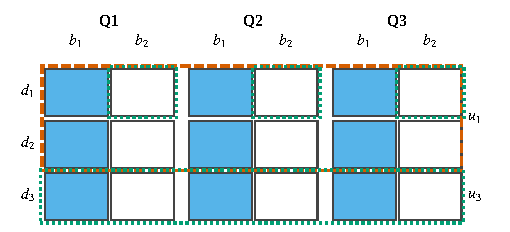
\includegraphics[width=\columnwidth]{fig_example.pdf}
\caption{One principal-independent entry serves three different scopes. One entry grouped by quarter and the policy attributes (department, brand); each cell holds a SUM and a COUNT. It serves three scopes: $u_1$ (dashed, departments $d_1,d_2$), $u_2$ (shaded, brand $b_1$), and $u_3$ (dotted, $(d_1\wedge b_2)\vee d_3$).}
\label{fig:example}
\Description{Diagram of a principal-independent cache entry grouped by quarter, department, and brand, and how three principals with different scopes derive answers from disjoint cells of the same entry.}
\end{figure}

\subsection{Lookup and derivation}

A call $q$ is \emph{derivable} from an entry $E$ when
(i) every base measure used by $M_q$ is in $\mathcal{M}_E$ with the current hash $h_{\Sigma_t}$;
(ii) every plain dimension of $G_q$ is in $G_E$, and every mapped dimension of $G_q$ has its source attribute in $G_E$;
(iii) for every filter $(A\in V_E)$ of $E$, $q$ has a filter $(A\in V_q)$ with $V_q\subseteq V_E$, and $A\in G_E$ if $V_q\neq V_E$; every filter of $q$ on an attribute that $E$ does not filter is on an attribute of $G_E$;
(iv) $W_q\subseteq W_E$, and $T\in G_E$ if $W_q\neq W_E$.
These are the roll-up, filter-push-down, and sub-range rules of view matching~\cite{goldstein01,deshpande98} with one more grouping dimension per policy attribute. Algorithm~\ref{alg:lookup} answers a call.

\begin{algorithm}[t]
\caption{ScopeCache lookup for call $(u,q)$ at time $t$}
\label{alg:lookup}
\KwIn{cache state $S$, policy $\pi_t$, snapshot $\Sigma_t$}
$\sigma\gets\scope_{\pi_t}(u)$;\ \lIf{$\Gamma_{\pi_t}(u)=\emptyset$}{\Return \M{NOGRANT}}
\lIf{$q$ needs a sensitive column $\notin C_{\pi_t}(u)$}{\Return \M{DENY}}
\If{$M_q$ has a non-decomposable metric}{\Return fallback($u,q$)}
\ForEach{entry $E\in S_*\cup S_\sigma$ (pinned views first)}{
  \If{$q$ derivable from $E$ under $\Sigma_t$}{
    $C\gets$ cells of $E$ satisfying $\psi_q$, $W_q$, and $\sigma$\tcp*{Lemma~\ref{lem:pure}}
    $Y\gets$ group $C$ by $G_q$ (mapped through $\mu_d$ of $\Sigma_t$), merge each $\mathit{agg}_b$\;
    \Return $f_m(Y)$ for $m\in M_q$ under $\Sigma_t$\;
  }
}
\Return miss($u,q$) \tcp*{Algorithm~\ref{alg:miss}}
\end{algorithm}

\begin{theorem}[Soundness and non-interference]
\label{thm:sound}
If $q$ is derivable from an entry $E$ that was computed on the current data, Algorithm~\ref{alg:lookup} returns $\mathit{Ans}_t(u,q)$, and its answer depends only on $D$ restricted to $\scope_{\pi_t}(u)$ and on the columns visible to $u$.
\end{theorem}
\begin{proof}
The checks in lines 1--2 use $\pi_t$ and coincide with those of the fresh execution. By (iii) and (iv), each residual filter and the window are predicates on attributes of $G_E$, and by Lemma~\ref{lem:pure} the scope is a predicate on attributes of $G_E$ too; hence the rows of $R$ that satisfy $\psi_q\wedge W_q\wedge\sigma$ are exactly the disjoint union of the rows of the selected cells $C$ (filters of $E$ are implied by those of $q$, so no qualifying row was excluded when $E$ was computed). SUM, COUNT, MIN, and MAX are distributive over disjoint unions (a merged sum over only NULL values stays NULL, as in SQL), and by (ii) the groups of $q$ are unions of groups of $G_E$, so merging $C$ by $G_q$ yields the base measures of the fresh query; by (i) they follow the current definitions, and line 9 applies the current formulas. For non-interference, the answer is a function of the cells in $C$, each of which aggregates only rows inside $\sigma$ by Lemma~\ref{lem:pure}; two instances that agree on the rows inside $\sigma$ have identical cells in $C$ and therefore identical answers. Hidden columns never reach the answer because line 2 rejects such calls. Equality is exact for COUNT, MIN, MAX, and integer sums, and holds up to the reassociation of floating-point additions otherwise; a fresh execution in a parallel engine has the same freedom.
\end{proof}

Here $S_*$ holds the shared entries and $S_\sigma$ the scope-keyed entries of the requester's normalized scope. The fallback for non-decomposable aggregates (line 3) keys the stored answer on the normalized scope, the request, and the definition hashes. Calls whose lifted entry would exceed the admission bound also store their answer under the normalized scope, and later calls of principals with the \emph{same} scope may derive from it by the rules above. Both are sound for the same reason as a scope-partitioned cache: the scope key is computed under $\pi_t$, so the entry was computed for exactly the requester's current scope.

\subsection{Miss path: predicate lifting and measure bundles}

A miss could store the requested answer, but then only principals with the same scope and nearly the same request could use it. ScopeCache instead executes a \emph{lifted} query that serves the requester and many future calls (Algorithm~\ref{alg:miss}). It groups by $G_q$ and all policy attributes and tries three liftings in order: the full history, the enclosing calendar years, and $W_q$ itself. The first two also move each filter on a policy attribute or on a dimension with at most 32 values into the grouping (and add the month when the window was widened); the third keeps the filters of $q$. Every lifting computes \emph{all} base measures of the fact table (a measure bundle), so that a later call for another metric of the same table also hits. ScopeCache takes the first lifting whose estimated size $\mathit{est}(G,W)$, the product of the domain sizes of the grouping attributes capped by the number of policy-value combinations present, is at most the admission bound $\min(B/10, B-B_{\mathit{pin}})$, where $B_{\mathit{pin}}$ is the space of pinned views. An entry that could not be admitted is never computed. If no lifting fits, the call takes the scope-keyed fallback path.

\begin{algorithm}[t]
\caption{ScopeCache miss for call $(u,q)$}
\label{alg:miss}
\ForEach{window $W\in\langle \text{full history}, \text{years}(W_q), W_q\rangle$}{
  $G\gets G_q\cup\mathcal{P}$\;
  \If{$W\neq W_q$}{$G\gets G\cup\{T\}\cup\{$filtered attributes with $\le 32$ values$\}$}
  $\psi\gets$ filters of $q$ on attributes $\notin G$\;
  \If{$\mathit{est}(G,W)\le\min(B/10,\,B-B_{\mathit{pin}})$}{
    $E\gets$ execute $P_E$ for $(G,\psi,W,$ all base measures$)$\;
    admit $E$ (evict by cost-aware GreedyDual~\cite{young94}); \Return lookup of $q$ on $E$\;
  }
}
\Return fallback($u,q$)\;
\end{algorithm}

Eviction follows GreedyDual with priority $L+\mathit{cost}\cdot\mathit{freq}/\mathit{size}$, where $\mathit{cost}$ is the number of fact-table rows that recomputing the entry scans, a deterministic proxy for its execution time, and $L$ the priority of the last victim~\cite{young94,lbsc24}; pinned views are never evicted.

\subsection{Permission events and republishes}

\begin{theorem}[Permission events need no invalidation]
\label{thm:events}
Membership moves, revocations, re-activations, grant edits, and column-grant edits require no invalidation of any entry, and the call immediately after such an event is answered according to the new policy.
\end{theorem}
\begin{proof}
Derivation entries contain no principal, no scope, and no column grant, so their content is the same under every policy state. Algorithm~\ref{alg:lookup} evaluates $\scope_{\pi_t}$ and $C_{\pi_t}$ on every call, and fallback keys are computed under $\pi_t$, so Theorem~\ref{thm:sound} applies to the first call after the event.
\end{proof}

\begin{assumption}
\label{ass:hash}
Definition hashes are collision-free: $h(b)=h(b')$ implies that $b$ and $b'$ are the same expression.
\end{assumption}

\begin{theorem}[Minimal invalidation on republish]
\label{thm:republish}
Under Assumption~\ref{ass:hash}, after a republish an entry column for base measure $b$ remains valid on every instance if $h_\Sigma(b)$ is unchanged, and changes of metric formulas, or of mappings of dimensions whose source attribute the entry stores, invalidate nothing. Among invalidation policies that observe definitions only through their hashes, no policy that is sound on every instance keeps a column whose hash changed.
\end{theorem}
\begin{proof}
Validity of unchanged columns follows from Theorem~\ref{thm:sound}. By Assumption~\ref{ass:hash} the stored aggregate is that of the current expression, and formulas and mappings are applied at lookup time under $\Sigma_t$. For minimality, if $h(b)$ changes, the old and new expressions differ syntactically; a policy that sees only hashes cannot distinguish this from a change that alters values on some instance, for example a new factor on a column that is non-zero in some cell, so keeping the column violates S1 on that instance.
\end{proof}

A mapped dimension whose source attribute has more than 32 values is stored as its mapped expression, tagged with the mapping version, and a republish of that mapping makes the column underivable. An online entry is dropped when all its measure columns are invalid and otherwise keeps serving the valid ones; a pinned view is recomputed only if one of its measures changed. A cache keyed on the snapshot identifier, as production metric layers stamp results, flushes everything instead.

\subsection{Pinned views selected under a budget}

When a prefix of the workload is available, ScopeCache pins views before serving. A candidate view is $P_E$ over the full history and all base measures, grouped by the attributes of one training grouping plus all policy attributes; its benefit is the number of fact-table rows that fresh executions of the training calls it derives would scan, and its cost is its row count. Selecting views under budget $B_v$ to maximize covered benefit is a budgeted maximum coverage problem.

\begin{proposition}[Selection]
\label{prop:select}
Over the calls of the training prefix, covered benefit is monotone submodular in the selected set. The better of the benefit-per-row greedy solution and the best single view that fits is within a factor $(1-1/e)/2$ of the optimal selection.
\end{proposition}
\begin{proof}
Benefit is a weighted coverage function, which is monotone and submodular; the bound is that of the modified greedy algorithm for budgeted maximum coverage~\cite{kmn99,celf07}.
\end{proof}

Pinned views and online entries share one budget: views are selected first and the remainder serves the online path. This generalizes greedy view selection on the data-cube lattice~\cite{hru96} with the policy attributes kept in every view. Without them, a view could not be filtered by a principal's scope; with them, a view built for one role serves every role.

\subsection{Holdout configuration and evidence-threshold unpinning}
\label{sec:adapt}

Pinned views and lifted online entries share one budget, and on a fine-grained policy the views can evict online entries that later callers would have reused. ScopeCache therefore chooses a configuration on the training prefix alone, and may unpin views when evicted online entries prove useful.

The training prefix---the same first 20\% used for view selection---is split: the first 75\% builds each candidate, and the last 25\% is a validation holdout that does not affect the measured suffix. The candidates are the raw-value hybrid (pinned views and online entries, the default), the online path alone, cells coarsened to grant-literal classes, and two variants that reserve 50\% or 30\% of the budget for the online path and may unpin views. The candidate with the fewest validation executions is used for the measured suffix; ties keep the default, which is first in the portfolio order. Validation never sees the measured calls.

A ghost directory records evicted online entries. A ghost hit grows the online reserve, up to $0.7B$. A pinned view is unpinned only after at least $\mathit{unpin\_min}=\unpinMinFrozen{}$ ghost hits; the threshold prevents unpinning on weak evidence. It was fixed after a development evaluation (seeds 0--2) in which unpinning with no threshold regressed on TPC-DS, and was then frozen. The fifteen-run headline of Section~\ref{sec:exp} uses this frozen configuration on unseen seeds; Section~\ref{sec:ablation} reports a sweep over $\{10,20,40,80\}$ as a sensitivity, not as a re-selection.

\subsection{Implementation and cost}
\label{sec:impl}
ScopeCache runs as a library between the metric tool and the warehouse. Entries are pandas frames over DuckDB results, grouped into one shared bucket (derivation entries and pinned views) and one bucket per scope key (fallback entries). A lookup tests the derivation conditions (i)--(iv) on each candidate, which needs only the entry's metadata, and then evaluates the scope on the policy columns of the candidate's cells with vectorized IN tests, one per literal of $\Gamma_\pi(u)$; with $n_E$ cells this costs $O(n_E\cdot|\Gamma_\pi(u)|\cdot k)$, plus a hash aggregation of the selected cells. The size of an entry is at most the number of policy-value combinations present in the data times the product of the domain sizes of its other grouping attributes, which is the estimate the admission bound uses. A miss issues one SQL statement that groups by the lifted attributes and computes the full measure bundle; a lifted execution groups by more attributes and may scan a wider window, so Section~\ref{sec:exp} also reports the fact-table rows that every cache scans.

\subsection{Discussion: cell granularity}
\label{sec:granularity}
Cells could be coarsened from raw policy values to the classes of values that no grant literal distinguishes (for attribute $P_j$, $v\equiv v'$ iff every value set in a literal on $P_j$ contains both or neither); Lemma~\ref{lem:pure} still holds for scopes over such literals. On our setups the variant (\M{SC-atoms}) stays within \atomsMeanSave\% of raw-value cells except on TPC-DS, and is cheaper on SYN-FG and ENT (Table~\ref{tab:ablation}). ScopeCache therefore keys cells on raw values, which also makes grant edits that introduce new value sets free.

\section{Experimental Evaluation}
\label{sec:exp}

We answer five questions. \textbf{RQ1}: Are all answers sound, and what do unsafe caches return? \textbf{RQ2}: How much warehouse work does ScopeCache save on rule-based multi-principal workloads? \textbf{RQ3}: How much cross-scope reuse do real LLM agents generate? \textbf{RQ4}: How do permission events and republishes affect reuse? \textbf{RQ5}: Which components matter, and what does ScopeCache cost?

\subsection{Setup}
\label{sec:setup}

\textbf{Setups.} Table~\ref{tab:setups} lists five fact tables built in DuckDB~\cite{duckdb19}: TPC-H (scale factor 1; lineitem joined with orders, customer, nation, region, part, and supplier)~\cite{tpch}, TPC-DS (scale factor 1; store sales with date, item, store, customer address, and demographics)~\cite{tpcds02}, the BIRD \emph{financial} database (transactions with accounts and districts)~\cite{bird23}, ENT, a synthetic reconstruction of an enterprise metric platform whose organization tree (813 departments, of which 456 leaves hold sales), grant modes, metric types, and query format follow the platform's code, with synthetic values only; and SYN-FG, which keeps the TPC-H scale-factor-1 fact table, adds a fully synthetic shop dimension of \synfgShops{} shops (twelve per nation, each shop consistent with its customers' nation), and assigns \synfgUsers{} principals through \synfgSharedGroups{} shared groups and \synfgSingletons{} singleton groups to \synfgScopes{} roles of the same five kinds (median \synfgMedian{} principal per scope, mean \synfgMean{}, at most \synfgMax{}), of which \synfgSensitivePct\% see the sensitive columns. Each setup has 6--8 base measures, 8--10 metrics including ratios and a COUNT DISTINCT, one mapped dimension, and one or two sensitive columns. TPC-H, TPC-DS, BIRD, and ENT have 400 principals mapped through 60 groups to roles of five kinds: hierarchical (for example, a region and its nations, or a department subtree), two-value, single-value, IN-product, and OR-of-conjuncts roles; 20--30\% of roles see the sensitive columns.

\begin{table}[t]
\centering
\caption{Scopes are fine-grained: every setup has 85--300 distinct scopes. Principals: 400 on TPC-H, TPC-DS, BIRD, and ENT; 700 on SYN-FG (60 shared groups and 240 singleton groups). Scopes counted at seed 0.}
\label{tab:setups}
\footnotesize
\setlength{\tabcolsep}{2.5pt}
\begin{tabular}{@{}lrrlr@{}}
\toprule
Setup & Rows & Months & Policy attributes (values) & Scopes\\
\midrule
TPC-H & 6.0M & 80 & nation, segm., mfgr (25$\times$5$\times$5) & 109\\
TPC-DS & 2.5M & 61 & state, category (51$\times$10) & 85\\
BIRD & 1.1M & 72 & district, freq. (77$\times$3) & 93\\
ENT & 2.0M & 36 & dept., brand, chan. (456$\times$12$\times$6) & 132\\
SYN-FG & 6.0M & 80 & shop, segm. (300$\times$5) & 300\\
\bottomrule
\end{tabular}
\end{table}


\textbf{Rule-based workloads.} Sessions imitate agent exploration: a monthly trend of a metric, followed by 2--8 actions drawn with weights 3 (break down by a dimension), 3 (drill into a value from the principal's own scope and break down by another dimension), 1.5 (switch metric), 1 (year-over-year), 1 (scalar), and 1 (retry). Principal activity follows a Zipf(0.8) distribution, metric popularity Zipf(0.9), and dimension popularity Zipf(0.7). Events occur per call with probability 0.004 (membership move), 0.002 (revocation), 0.001 (re-activation), 0.002 (grant edit), 0.001 (column-grant edit), and 0.001 (republish of a measure, a formula, or a mapping); after 50\% of permission events, the affected principal immediately replays its previous call, which tests the zero staleness window adversarially. Each setup runs three seeds of 3{,}000 calls; the first 20\% warm the caches and train the views, and metrics are computed on the remaining 80\%. The headline grid (Table~\ref{tab:main}) uses seeds 3, 4, and 5, which were not used to design the method or to choose $\mathit{unpin\_min}$; that configuration, including $\mathit{unpin\_min}=\unpinMinFrozen{}$, was frozen beforehand. Development work used seeds 0--2 and is reported only as such. Warehouse execution counts are deterministic under a machine-independent eviction-cost model; we do not mix wall-clock times across machines. Confidence intervals on total-execution differences are paired bootstraps over cells (\bootB{} replicates, seed \bootSeed{}), reported as analysis of the already collected headline, not as a second evaluation. A pre-registered robustness evaluation on unseen seeds 6--10, including a shifted workload declared beforehand, is in Table~\ref{tab:rob} and does not replace Table~\ref{tab:main}.

\textbf{Agent traces.} Tool-calling agents answer 20 business questions per setup (for example, ``which channels have the highest refund rate this year, and is it rising?''), written before any recording to cover each setup's metrics and dimensions and released with the traces, for 40 principals with five questions each, through three tools: listing dimension values, a metric query (1--3 metrics, at most two dimensions, IN filters, a month range), and a final answer, with at most six tool calls. The warehouse applies the principal's row scope. We use deepseek-chat (DeepSeek), GLM-4.5-flash (Zhipu AI), and Kimi-K2.6 (Moonshot AI) through the vendors' APIs at temperature 0 (Kimi: 0.6, the only value its endpoint accepts), accessed November 7--10, 2026, with two recording seeds that draw different principals and policies, and GPT-6 (gpt-6-sol, OpenAI) and Claude Opus~5.5 (Anthropic) through the tokens1688 gateway on November 11, 2026, with one recording seed at their default reasoning settings (\nAgentTraces{} traces, \nAgentCalls{} metric calls; \$\agentCost{} at list prices for the vendor APIs and \intlMTokens{}M tokens through the gateway). Only public and synthetic data reach the models. Traces are replayed through every cache with the same differential test; as in the rule-based runs, the first 20\% of each trace train the views and warm the caches, and metrics are computed on the \nAgentDataCalls{} data calls after the prefix (the other metric calls are in the prefix or are rejected).

\textbf{Baselines.} \M{NoCache} (the production setting); \M{Exact}, keyed on the rewritten SQL including the row predicate and the metric definitions (like a warehouse result cache~\cite{snowflake16}); \M{PerUser}; \M{PerScope}, keyed on the normalized scope, which is a scope-aware semantic cache with roll-up and filter derivation; \M{TTL}, a per-user cache whose entries expire after 500 calls and are served without re-checking the current policy (a miss executes under the current policy); \M{SemNoScope}, an intent-keyed OLAP semantic cache with roll-up and filter push-down that ignores the requester~\cite{bindschaedler26}; \M{ViewRewrite}, views selected offline by benefit-per-row greedy over the same training prefix and filtered by the scope at query time (VPD over views~\cite{rizvi04,hru96}), with views recomputed when a measure changes, as BI aggregate-awareness layers route queries to pre-aggregates and apply access filters; \M{VR-adapt}, which re-selects its views every 600 calls on the last 600 calls and materializes the newly selected views as warehouse executions; and \M{PerScope+}, which uses ScopeCache's lifting, measure bundles, and hash-based invalidation but computes each entry for the requester's scope and shares it only within that scope, isolating the effect of cross-scope sharing; \M{PerScope+V} adds ScopeCache's pinned views to \M{PerScope+}. \M{ViewRewrite} executes calls that its views do not cover. The request-, user-, and scope-keyed caches flush on every snapshot change, as results stamped with a snapshot identifier are. All caches have a budget of $B=10^6$ rows, use the same derivation code, and run in one process. In the tables that follow, ScopeCache denotes the full system of Section~\ref{sec:adapt}, and \M{SC-hybrid} denotes the same cache with a fixed raw-value hybrid configuration, without holdout selection or POP.

\textbf{Metrics.} Every answer of every method is compared value by value with a fresh execution under the requester's current policy and snapshot (relative tolerance $10^{-6}$); a wrong answer is \emph{over-privileged} if it uses rows outside the requester's scope, and \emph{stale} otherwise. Whether an agent chooses the right query for a question is orthogonal to caching: every cache replays the same calls, so it is identical across methods. The oracle aggregates in SQL and applies metric formulas in Python; an independent oracle that evaluates the formulas in SQL agreed with it on \oracleAgree{} of \oracleChecked{} sampled calls under the policy and snapshot current at each call. We report the hit rate over data calls and the number of warehouse executions, the cost the problem minimizes, including view rebuilds after a republish and view re-selections, together with the fact-table rows that these executions scan; the initial materialization of pinned views on the training prefix is not counted, just as the training calls of the online caches are not; each avoided execution saves a warehouse call, which costs about 0.5\,s at the median on the production platform (connection, snapshot fetch, and query). Eviction priorities and view benefits use the number of fact-table rows a re-computation scans, so warehouse executions are machine-independent and deterministic for a given seed; the per-hit derivation time was measured in separate runs (Section~\ref{sec:ablation}). In every results table, the best value is in bold and the second best underlined, ranked by the printed value so that ties share the mark (higher hit rates and fewer executions or wrong answers are better); the unsafe \M{TTL} and \M{SemNoScope} are not ranked. The original runs on TPC-H, TPC-DS, BIRD, and ENT, and the timing and agent-trace measurements, ran on an Apple M4 (10 cores) with DuckDB 1.4.5; the SYN-FG execution counts were obtained with the same deterministic cost model on a different machine and are comparable. We do not mix wall-clock times across machines.

\subsection{RQ1: Soundness}
\label{sec:rq1}

\textbf{Standing.} ScopeCache is best, tied with the other safe caches, in all four wrong-answer columns of Table~\ref{tab:safety}: no wrong answer in \nMainDataCalls{} rule-based and \nAgentDataCalls{} agent data calls.

\begin{table}[t]
\centering
\caption{Only the two shared caches are unsafe; no safe cache returns a wrong answer. Wrong answers on the development grid (seeds 0--2, \nMainDataCalls{} data calls) and the agent traces. On the unseen-seed headline grid, ScopeCache, \M{SC-hybrid}, and \M{PerScope+V} also returned no wrong answer (\freshDataCalls{} data calls).}
\label{tab:safety}
\footnotesize
\setlength{\tabcolsep}{4pt}
\begin{tabular}{@{}lrrrrr@{}}
\toprule
 & \multicolumn{3}{c}{Main grid} & \multicolumn{2}{c}{Agent traces}\\
\cmidrule(lr){2-4}\cmidrule(l){5-6}
Method & Data calls & Wrong & Over-priv. & Wrong & Over-priv.\\
\midrule
\M{Exact} & 31{,}273 & \textbf{0} & \textbf{0} & \textbf{0} & \textbf{0}\\
\M{PerUser} & 31{,}273 & \textbf{0} & \textbf{0} & \textbf{0} & \textbf{0}\\
\M{PerScope} & 31{,}273 & \textbf{0} & \textbf{0} & \textbf{0} & \textbf{0}\\
\M{PerScope+} & 31{,}273 & \textbf{0} & \textbf{0} & \textbf{0} & \textbf{0}\\
\M{PerScope+V} & 31{,}273 & \textbf{0} & \textbf{0} & \textbf{0} & \textbf{0}\\
\M{TTL} & 31{,}273 & 39 & 12 & -- & --\\
\M{SemNoScope} & 31{,}273 & 8{,}670 & 7{,}571 & 8{,}004 & 6{,}851\\
\M{ViewRewrite} & 31{,}273 & \textbf{0} & \textbf{0} & \textbf{0} & \textbf{0}\\
\M{VR-adapt} & 31{,}273 & \textbf{0} & \textbf{0} & \textbf{0} & \textbf{0}\\
\M{SC-hybrid} & 31{,}273 & \textbf{0} & \textbf{0} & \textbf{0} & \textbf{0}\\
\M{SC-online} & 31{,}273 & \textbf{0} & \textbf{0} & \textbf{0} & \textbf{0}\\
\M{SC-nolift} & 31{,}273 & \textbf{0} & \textbf{0} & -- & --\\
\M{SC-snap} & 31{,}273 & \textbf{0} & \textbf{0} & -- & --\\
\M{SC-atoms} & 31{,}273 & \textbf{0} & \textbf{0} & \textbf{0} & \textbf{0}\\
\bottomrule
\end{tabular}
\end{table}


Table~\ref{tab:safety} counts wrong answers over the development grid (seeds 0--2, \nMainDataCalls{} data calls) and all agent traces. ScopeCache, its variants, and the partitioned caches each answered those calls without a wrong answer (\nSafeDataCalls{} rule-based answers over all \nSafeCachesWord{} safe caches), including every adversarial replay right after a revocation. On the unseen-seed headline grid, ScopeCache, \M{SC-hybrid}, and \M{PerScope+V} similarly returned no wrong answer on \freshDataCalls{} data calls. The two shared caches did not: \M{SemNoScope} returned over-privileged answers in \semOverLo--\semOverHi\% of data calls, and \M{TTL}, whose entries outlive permission changes, returned wrong answers to \ttlReplayWrong{} of \ttlReplayCalls{} adversarial replays at the 16-fold event rate. Sharing without a permission-independent entry format is therefore not an option, and the remaining questions compare ScopeCache with the safe caches.

\Takeaway{On \nMainDataCalls{} rule-based and \nAgentDataCalls{} agent data calls, every ScopeCache answer equaled a fresh execution under the current policy, including the first call after each revocation.}

\subsection{RQ2: Efficiency on multi-principal workloads}
\label{sec:rq2}

\textbf{Standing.} On fifteen runs whose seeds were held out from design and from the choice of $\mathit{unpin\_min}$, ScopeCache matches or beats \M{PerScope+V} in every cell: \psvW{} wins, \psvT{} ties, \psvL{} losses (Table~\ref{tab:main}). It needs \freshRedTot\% fewer warehouse executions in total (\freshOursTot{} against \freshPSVTot{}, a difference of \freshDeltaPsv{}; \M{SC-hybrid} totals \freshHybTot{}, a difference of \freshDeltaHyb{}). A paired bootstrap that resamples the 15 cells (\bootB{} replicates, seed \bootSeed{}) gives a 95\% CI of [\freshCIpsvLo{}, \freshCIpsvHi{}] for the total-execution difference versus \M{PerScope+V} and [\freshCIhybLo{}, \freshCIhybHi{}] versus \M{SC-hybrid}; both exclude zero ($p\freshPpsv{}$ and $p=\freshPhyb{}$).

\begin{table*}[t]
\centering
\caption{Headline evaluation on fifteen runs whose seeds (3, 4, 5) were held out from design and from the choice of $\mathit{unpin\_min}$. ScopeCache matches or beats \M{PerScope+V} in every cell: 10 wins, 5 ties, 0 losses. Warehouse executions; bold is best and underline is second among the three methods, with ties sharing the mark. W--T--L is versus \M{PerScope+V}. \M{SC-hybrid} is the same cache with a fixed raw-value hybrid configuration (no holdout, no POP). ScopeCache is the full system (holdout selection and evidence-threshold POP, $\mathit{unpin\_min}=40$, frozen before these runs). The \emph{Chosen} row is the holdout decision of ScopeCache ($\mathit{raw}$: raw-value hybrid; $\mathit{atoms}$: grant-literal cells; $\mathit{pop50}$/$\mathit{pop30}$: POP with a 50\% or 30\% online reserve). On TPC-H seed 3, ScopeCache is second to \M{SC-hybrid} (348 vs.\ 328) and still ahead of \M{PerScope+V} (352).}
\label{tab:main}
\footnotesize
\setlength{\tabcolsep}{2.5pt}
\begin{tabular}{@{}lrrrrrrrrrrrrrrrc@{}}
\toprule
 & \multicolumn{3}{c}{TPC-H} & \multicolumn{3}{c}{TPC-DS} & \multicolumn{3}{c}{BIRD} & \multicolumn{3}{c}{ENT} & \multicolumn{3}{c}{SYN-FG} & \\
\cmidrule(lr){2-4}\cmidrule(lr){5-7}\cmidrule(lr){8-10}\cmidrule(lr){11-13}\cmidrule(lr){14-16}
Method & 3 & 4 & 5 & 3 & 4 & 5 & 3 & 4 & 5 & 3 & 4 & 5 & 3 & 4 & 5 & W--T--L\\
\midrule
\M{SC-hybrid} & \textbf{328} & \underline{312} & \underline{398} & \textbf{228} & \textbf{243} & \textbf{255} & \textbf{193} & \textbf{164} & \textbf{223} & \underline{168} & \textbf{150} & \underline{201} & 665 & 635 & 650 & 6--6--3\\
\M{PerScope+V} & 352 & 328 & 405 & \textbf{228} & \underline{250} & \underline{259} & \textbf{193} & \textbf{164} & \textbf{223} & \underline{168} & \textbf{150} & \underline{201} & \underline{659} & \underline{605} & \underline{619} & ---\\
\textbf{ScopeCache} & \underline{348} & \textbf{264} & \textbf{323} & \textbf{228} & \textbf{243} & \textbf{255} & \textbf{193} & \textbf{164} & \textbf{223} & \textbf{167} & \textbf{150} & \textbf{197} & \textbf{638} & \textbf{541} & \textbf{578} & \textbf{10--5--0}\\
\midrule
Chosen & raw & pop50 & pop50 & raw & raw & raw & raw & raw & raw & atoms & raw & atoms & pop50 & pop30 & pop30 & \\
\bottomrule
\end{tabular}
\end{table*}


Table~\ref{tab:main} is the headline evaluation. The method, including $\mathit{unpin\_min}=\unpinMinFrozen{}$, was frozen before these runs (Section~\ref{sec:adapt}). ScopeCache is best or tied for best in 14 of the 15 cells. The one second-best cell is TPC-H seed 3: 348 executions against 328 for \M{SC-hybrid} and 352 for \M{PerScope+V}. The selector kept the raw-value hybrid: on the \lossValCalls{}-call validation slice, that configuration and grant-literal cells tied at 16 executions, ahead of $\mathit{pop30}$ (18) and $\mathit{pop50}$ (19), and the portfolio order kept the default. Validation is too short to accumulate $\mathit{unpin\_min}=\unpinMinFrozen{}$ ghost hits, so it compared a still-pinned hybrid with the reserved-budget candidates. On the measured suffix, \lossGhost{} ghost hits crossed the threshold and POP unpinned \lossUnpins{} views (\lossUnpinRows{} rows); view hits fell from \lossHitViewHyb{} to \lossHitViewOurs{}, which costs \lossExtraExec{} executions against not unpinning---a 1.1\% lead over \M{PerScope+V} and a 6.1\% deficit against \M{SC-hybrid}. At $\mathit{unpin\_min}=80$ on this same cell, 72 ghost hits do not unpin, and the run is identical to \M{SC-hybrid} (328 executions, the same \lossHitViewHyb{} view hits); we do not adopt 80 (Table~\ref{tab:sens}). This is the only loss against the non-adaptive hybrid (\scVsHybWTL{}), and the only raw-hybrid cell of the eight on the headline grid in which ghost hits reached 40.

Against \M{PerScope+V}, the three SYN-FG cells---the setting on which \M{SC-hybrid} itself needs more executions (665, 635, and 650 against 659, 605, and 619; \hybWTL{})---become wins of 3.2\%, 10.6\%, and 6.6\% (638, 541, and 578). The holdout selected a POP configuration with a 50\% or 30\% online reserve, which is the response to the view--online budget competition that had left the hybrid behind. The largest leads are on TPC-H seeds 4 and 5 (19.5\% and 20.2\%), where it selected $\mathit{pop50}$. On BIRD, and on ENT seed 4 and TPC-DS seed 3, the three methods tie: pinned views already cover the shareable calls, and the selector correctly kept the default hybrid. On ENT seeds 3 and 5 it selected grant-literal cells and needs 0.6\% and 2.0\% fewer executions than both other methods. Every run has $\mathit{wrong}=0$. Hit rates of ScopeCache are \freshHitLo--\freshHitHi\% over the 15 runs.

On the development grid (seeds 0--2), \M{SC-hybrid} already needed \redVRLo--\redVRHi\% fewer executions than \M{ViewRewrite} in all 15 runs and \redPSmainLo--\redPSmainHi\% fewer than \M{PerScope}; we do not combine those seeds with the headline. Fig.~\ref{fig:breakdown} attributes each \M{SC-hybrid} hit on that development grid: pinned views serve \bdViewLo--\bdViewHi\% of data calls, and entries created by other principals \bdOtherLo--\bdOtherHi\%, almost all of them under a different scope.

\Takeaway{On seeds held out from design, ScopeCache matches or beats the strongest baseline in all 15 runs (\psvW--\psvT--\psvL) and turns the three SYN-FG losses of the non-adaptive hybrid into wins; it is second in one TPC-H cell, where it still leads \M{PerScope+V}.}

\begin{figure}[t]
\centering
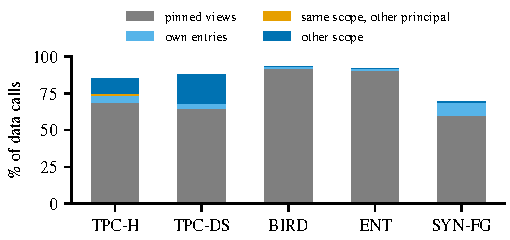
\includegraphics[width=\columnwidth]{fig_breakdown.pdf}
\caption{Pinned views and entries shared across scopes supply the hits of the core cache; the hits a scope-partitioned cache could also obtain are \bdSelfSameLo--\bdSelfSameHi\% of data calls. Source of each \M{SC-hybrid} hit on the development grid (seeds 0--2), as a share of data calls (mean of three seeds).}
\label{fig:breakdown}
\Description{Stacked breakdown of SC-hybrid hits on the development workloads, distinguishing pinned views, entries shared across scopes, and hits a scope-partitioned cache could also obtain.}
\end{figure}

\subsection{RQ3: Real LLM agents}
\label{sec:rq3}

\textbf{Standing.} The hybrid configuration is best in \agBestCells{} of the \agCells{} hit-rate and execution cells of Table~\ref{tab:agent}. Agent traces use \M{SC-hybrid}; they were not rerun with holdout selection.

\begin{table*}[t]
\centering
\caption{ScopeCache has the highest hit rate and the fewest executions on every setup of the agent traces. X-sc.: cross-scope share of \M{SC-online}; abbreviations in Section~\ref{sec:rq3}.}
\label{tab:agent}
\footnotesize
\setlength{\tabcolsep}{4pt}
\begin{tabular}{@{}lrrrrrrrrrrrrr@{}}
\toprule
 & & & \multicolumn{5}{c}{Hit rate (\%)} & & \multicolumn{5}{c}{Executions}\\
\cmidrule(lr){4-8}\cmidrule(l){10-14}
Setup & Traces & Data calls & PS & PS+ & PS+V & VR & SC & X-sc. & PS & PS+ & PS+V & VR & SC\\
\midrule
TPC-H & 8 & 2{,}462 & 32.8 & 66.3 & \underline{90.1} & 85.7 & \textbf{97.4} & 93.4 & 203.6 & 101.5 & \underline{29.6} & 44.1 & \textbf{7.8}\\
TPC-DS & 8 & 2{,}318 & 29.2 & 71.6 & \underline{95.5} & 95.2 & \textbf{96.9} & 92.3 & 203.5 & 81.2 & \underline{13.1} & 14.1 & \textbf{9.4}\\
BIRD & 8 & 2{,}014 & 34.6 & 61.5 & \textbf{96.5} & \underline{95.9} & \textbf{96.5} & 91.5 & 161.5 & 94.9 & \textbf{8.8} & \underline{10.2} & \textbf{8.8}\\
ENT & 8 & 2{,}370 & 29.9 & 38.4 & \textbf{98.1} & \underline{97.8} & \textbf{98.1} & 38.1 & 205.2 & 180.8 & \textbf{5.6} & \underline{6.5} & \textbf{5.6}\\
\midrule
Best/2nd & & & 0/0 & 0/0 & 2/2 & 0/2 & 4/0 & & 0/0 & 0/0 & 2/2 & 0/2 & 4/0\\
\bottomrule
\end{tabular}
\end{table*}


Table~\ref{tab:agent} and Fig.~\ref{fig:agent} replay the recorded traces (in Table~\ref{tab:agent}, PS, PS+, PS+V, VR, and SC abbreviate \M{PerScope}, \M{PerScope+}, \M{PerScope+V}, \M{ViewRewrite}, and ScopeCache, other columns are means per trace, and data calls are totals over the traces of a setup); we attribute hits to their creators with the configuration without pinned views (\M{SC-online}), because a view serves calls of all principals. Agents issue \agentCallsPerEpLo--\agentCallsPerEpHi{} metric calls per question in a trace, and their calls repeat across principals: ScopeCache serves \agentXscopeLo--\agentXscopeHi\% of data calls from entries created under a different scope, and needs \redPSLo--\redPSHi\% fewer executions than \M{PerScope}, at hit rates of \agentScHitLo--\agentScHitHi\% (\M{ViewRewrite}: \agentVRHitLo--\agentVRHitHi\%; \M{VR-adapt} coincides with it because every trace is shorter than its re-selection period); ScopeCache needs \agentRedVRmed\% fewer executions than \M{ViewRewrite} at the median over traces, and its online variant, which receives no training prefix, needs \agentRedOnlinePSLo--\agentRedOnlinePSHi\% fewer than \M{PerScope}. \agentPSVSentence{} Cross-scope reuse is lowest on ENT (\agentXscopeEntD\%); with a budget of $10^7$ rows it rises to \entBigXscope\%, so the admission bound, not the workload, limits it there (Section~\ref{sec:ablation}).

\begin{figure}[t]
\centering
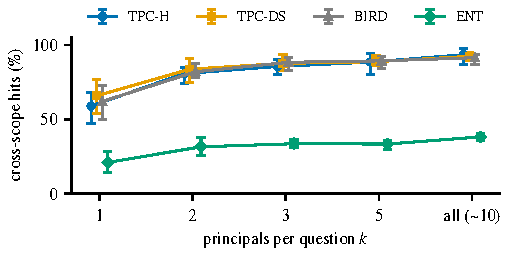
\includegraphics[width=\columnwidth]{fig_sens.pdf}
\caption{Cross-scope reuse persists when no two principals ask the same question ($k=1$) and grows with question overlap. Cross-scope reuse on agent traces when each question is asked by only the first $k$ principals assigned to it (\M{SC-online}; mean over vendors and recording seeds; whiskers: range).}
\label{fig:sens}
\Description{Line chart of cross-scope reuse on agent traces as the number of principals who ask the same question grows from one to many.}
\end{figure}

\textbf{Agent models.} The \nModelsWord{} models explore differently, from \callsPerQLo{} to \callsPerQHi{} metric calls per question (Table~\ref{tab:agentvendor}, which aggregates each model over all setups and recording seeds and is not ranked because its rows are models, not methods). Cross-scope reuse is high for every model, and no safe cache returned a wrong answer on any trace. The intent-keyed \M{SemNoScope} reaches hit rates of \agentSemHitLo--\agentSemHitHi\% on these traces, but \agentSemOverLo--\agentSemOverHi\% of its data calls return another principal's result (Table~\ref{tab:safety}).

\begin{table}[t]
\centering
\caption{Cross-scope reuse and the savings over \M{PerScope} hold for every agent model. Exec. ratio: ScopeCache executions over those of \M{PerScope}.}
\label{tab:agentvendor}
\footnotesize
\setlength{\tabcolsep}{4pt}
\begin{tabular}{@{}lrrrr@{}}
\toprule
Model & Calls/q. & Hit (\%) & X-sc. (\%) & Exec. ratio\\
\midrule
deepseek-chat & 1.73 & 97.1 & 78.6 & 0.038\\
GLM-4.5-flash & 2.19 & 97.2 & 77.5 & 0.044\\
Kimi-K2.6 & 2.47 & 96.9 & 79.1 & 0.051\\
GPT-6 (gpt-6-sol) & 1.79 & 97.7 & 80.4 & 0.032\\
Claude Opus 5.5 & 1.82 & 97.8 & 79.8 & 0.032\\
\bottomrule
\end{tabular}
\end{table}


\textbf{When do principals share questions?} In our traces each question is assigned to about ten principals. Fig.~\ref{fig:sens} keeps only the first $k$ principals per question. With a single principal per question ($k=1$; \sensOneCalls{} data calls over the \nAgentTraces{} traces), every cross-scope hit reuses an entry created for a \emph{different} question, as is or by roll-up, filtering, or sub-ranging; ScopeCache still serves \sensOneLo--\sensOneHi\% of data calls from other scopes (\sensOneTpch\% on TPC-H; \sensOneEnt\% on ENT, the setup with the largest policy domain, 456 departments), and the share rises to \sensTwoLo--\sensTwoHi\% at $k=2$.

\Takeaway{Real agents generate cross-scope reuse: \agentXscopeMeanLo--\agentXscopeMeanHi\% of their data calls are answered exactly from aggregates computed for another scope, and \sensOneLo--\sensOneHi\% even when no two principals ask the same question.}

\subsection{RQ4: Permission events and republishes}
\label{sec:rq4}

\textbf{Standing.} On SYN-FG, the fine-grained setting, ScopeCache needs \evSynfgRedLo--\evSynfgRedHi\% fewer executions than \M{PerScope+V} at every event rate (Table~\ref{tab:events}; 4 wins, 0 ties, 0 losses). These four cells use development seed 0 with common random numbers and are not part of the unseen-seed headline.

\begin{table}[t]
\centering
\caption{On SYN-FG at four event rates (development seed 0, common random numbers; \emph{not} part of the unseen-seed headline), ScopeCache needs 9.2--14.3\% fewer executions than \M{PerScope+V} (4 wins, 0 ties, 0 losses). The holdout selected $\mathit{pop30}$ at every rate. The sixteen public-setup event cells were measured with \M{SC-hybrid} and were not rerun with the full system; under that configuration ScopeCache was already best or tied on those cells. Warehouse executions and hit rate (\%); bold is best.}
\label{tab:events}
\footnotesize
\setlength{\tabcolsep}{3.6pt}
\begin{tabular}{@{}lrrrr@{}}
\toprule
 & $0\times$ & $1\times$ & $4\times$ & $16\times$\\
\midrule
\M{PerScope+V} exec. & 643 & 649 & 676 & 704\\
\textbf{ScopeCache} exec. & \textbf{551} & \textbf{571} & \textbf{614} & \textbf{611}\\
Relative reduction & 14.3\% & 12.0\% & 9.2\% & 13.2\%\\
\midrule
\M{PerScope+V} hit & 69.9 & 69.7 & 68.7 & 68.2\\
\textbf{ScopeCache} hit & \textbf{74.2} & \textbf{73.3} & \textbf{71.3} & \textbf{71.7}\\
\bottomrule
\end{tabular}
\end{table}


Table~\ref{tab:events} scales all event probabilities by 0, 1 (the default), 4, and 16: every rate issues the same 3{,}000 calls, the events at a higher rate include those at a lower rate, and the adversarial replays that permission events trigger come on top. The holdout selected $\mathit{pop30}$ at every rate. As Theorems~\ref{thm:events} and~\ref{thm:republish} predict, events change ScopeCache's reuse little: its hit rate at $16\times$ is 71.7\% against 74.2\% with no events. The sixteen public-setup event cells were measured with \M{SC-hybrid} and were not rerun with the full system; under that configuration ScopeCache was already best or tied, and its hit rate at 16 times the default rates differed from the event-free run by at most \evHitDropMax{} points. \M{SC-snap}, which is the core cache keyed on the snapshot identifier, needs \snapFactorLo--\snapFactorHi$\times$ the executions of the hybrid at the default rate (Table~\ref{tab:ablation}) and up to \snapFactorSixteen$\times$ at 16 times, because it flushes on every snapshot change.

\Takeaway{Permission events cost ScopeCache no invalidation, and a republish only the changed measure columns; on SYN-FG the full system leads \M{PerScope+V} at every event rate, and flushing on snapshot changes multiplies warehouse executions by up to \snapFactorSixteen$\times$.}

\subsection{RQ5: Ablation, robustness, and overhead}
\label{sec:ablation}

\textbf{Standing.} Removing any component of the core cache costs executions on at least one setup (Table~\ref{tab:ablation}, development seeds, relative to \M{SC-hybrid}). On the unseen-seed headline, the frozen unpinning threshold is necessary for the comparison with \M{PerScope+V} (Table~\ref{tab:sens}). A later pre-registered evaluation on unseen seeds 6--10, including a declared workload shift, is in Table~\ref{tab:rob}; it does not replace the headline of Table~\ref{tab:main}.

\begin{table}[t]
\centering
\caption{Removing any component of the core cache costs executions on at least one setup (development seeds 0--2). Executions relative to \M{SC-hybrid}; G.\,mean: geometric mean over setups. These are not the headline numbers of Table~\ref{tab:main}. $^\dagger$Relative to \M{SC-online}, seed 0.}
\label{tab:ablation}
\footnotesize
\setlength{\tabcolsep}{3.6pt}
\begin{tabular}{@{}lrrrrr@{\hspace{7pt}}r@{}}
\toprule
Variant & TPC-H & TPC-DS & BIRD & ENT & SYN-FG & G.\,mean\\
\midrule
\M{SC-hybrid} & \textbf{1.00$\times$} & \textbf{1.00$\times$} & \textbf{1.00$\times$} & \underline{1.00$\times$} & 1.00$\times$ & \textbf{1.00$\times$}\\
\M{SC-online} & 1.11$\times$ & 1.22$\times$ & \underline{1.60$\times$} & 4.30$\times$ & \textbf{0.96$\times$} & 1.55$\times$\\
\M{PerScope+} & 2.38$\times$ & 2.38$\times$ & 3.36$\times$ & 5.65$\times$ & 1.31$\times$ & 2.69$\times$\\
\M{SC-nolift} & \underline{1.03$\times$} & \underline{1.04$\times$} & \textbf{1.00$\times$} & \underline{1.00$\times$} & 1.01$\times$ & \underline{1.02$\times$}\\
\M{SC-snap} & 1.19$\times$ & 1.33$\times$ & 1.70$\times$ & 4.18$\times$ & 1.01$\times$ & 1.63$\times$\\
\M{SC-atoms} & \textbf{1.00$\times$} & 1.05$\times$ & \textbf{1.00$\times$} & \textbf{0.99$\times$} & \underline{0.97$\times$} & \textbf{1.00$\times$}\\
\midrule
\M{SC-online-nolift}$^\dagger$ & 1.45$\times$ & 1.29$\times$ & 1.85$\times$ & 1.00$\times$ & 1.28$\times$ & 1.35$\times$\\
\bottomrule
\end{tabular}
\end{table}


Table~\ref{tab:ablation} removes one component at a time on the development grid (seeds 0--2, means of three seeds), relative to \M{SC-hybrid}; those absolute executions are not the headline numbers of Table~\ref{tab:main}. Without pinned views (\M{SC-online}), the hybrid needs \onlineFactorLo--\onlineFactorHi$\times$ the executions of \M{SC-hybrid}. The factor is largest on ENT (\onlineFactorEnt$\times$), whose 456 departments make lifted entries exceed the admission bound, so that pinned views supply the coverage there and the online path supplies it where the training prefix did not anticipate the calls. It is \onlineFactorLo$\times$ on SYN-FG: the default budget evicts more of the hybrid's online entries than of \M{SC-online}, so pinning views costs \synfgOnlineVsSCLo--\synfgOnlineVsSCHi\% executions there relative to \M{SC-online}. Partitioning the online entries by scope (\M{PerScope+}) multiplies executions further. Predicate lifting pays off on the online path, where it saves \onlineNoliftSaveLo--\onlineNoliftSaveHi\% of executions (\M{SC-online-nolift}) on every setup except ENT, for that reason; with pinned views, which already hold the lifted groupings of the training prefix, \M{SC-nolift} stays within \noliftAbsMax\% of \M{SC-hybrid}. Coarsening cells to grant-literal classes (\M{SC-atoms}) needs \atomsMeanWorse\% more executions on TPC-DS and stays within \atomsMeanSave\% elsewhere, which motivates keying cells on raw values (Section~\ref{sec:granularity}); it is \atomsMeanSave\% cheaper on ENT (\atomsEntExecDiff{} executions, against a standard deviation of \scEntExecSd{} over seeds) because coarser cells keep more lifted entries under the admission bound (\atomsEntFbRed\% fewer calls take the scope-keyed path). Without lifting, a miss scans only the requested window: on \rowsUnfSetup, \M{SC-nolift} scans \noliftRowsRedVR\% fewer rows than \M{ViewRewrite} and needs \noliftExecRedVR\% fewer executions.

\textbf{Unpinning threshold.} Table~\ref{tab:sens} varies $\mathit{unpin\_min}$ among 10, 20, 40, and 80 on the same fifteen unseen-seed runs, every other part of the frozen method held fixed. This is a sensitivity sweep, not a re-selection: 10 and 20 fail versus \M{PerScope+V} (7--4--4 and 8--5--2) by unpinning on weak ghost evidence; 80 also yields 10--5--0 and 34 fewer executions, an advantage observed after the freeze, and is not adopted. The official totals remain \freshOursTot{} at $\mathit{unpin\_min}=\unpinMinFrozen{}$.

\begin{table}[t]
\centering
\caption{Sensitivity of $\mathit{unpin\_min}$ on the same fifteen unseen-seed runs, reported as a sensitivity sweep, not as threshold selection. The official method uses 40, frozen before these runs. Thresholds 10 and 20 lose to \M{PerScope+V} on some cells (the same weak-evidence unpinning that motivated the freeze). A threshold of 80 also yields 10--5--0 and 34 fewer executions in total---an advantage observed after the freeze---and is not adopted. W--T--L is versus \M{PerScope+V}; $\Delta$ is versus the frozen total of 4{,}512.}
\label{tab:sens}
\footnotesize
\setlength{\tabcolsep}{3.4pt}
\begin{tabular}{@{}rrrrrrr@{}}
\toprule
$\mathit{unpin\_min}$ & W & T & L & Exec. & vs.\ PSV & $\Delta$\\
\midrule
10 & 7 & 4 & 4 & 4{,}557 & 5.1\% & $+45$\\
20 & 8 & 5 & 2 & 4{,}561 & 5.1\% & $+49$\\
\textbf{40 (official)} & \textbf{10} & \textbf{5} & \textbf{0} & \textbf{4{,}512} & \textbf{6.1\%} & ---\\
80 & 10 & 5 & 0 & 4{,}478 & 6.8\% & $-34$\\
\bottomrule
\end{tabular}
\end{table}


\textbf{Interest drift and budget.} When metric and dimension popularity are reshuffled every 30 sessions, the training prefix no longer matches the workload, and \M{SC-hybrid} needs \driftRedLo--\driftRedHi\% fewer executions than \M{ViewRewrite} (development seed 0). With a budget of $10^5$ rows, \M{SC-hybrid} needs \smallRedLo--\smallRedHi\% fewer; the high end is SYN-FG, where the views of \M{ViewRewrite} no longer fit and that baseline executes every data call, and at this tighter budget the hybrid also needs fewer executions than \M{PerScope+V} on SYN-FG.

\textbf{Policy-domain size.} To see how sharing scales with the granularity of grants, a synthetic fact table has one policy attribute with 50 to 3{,}000 values and 400 principals with random value sets (median about 5\% of the values), so that from 300 values on nearly every principal has its own scope (Fig.~\ref{fig:domain}). Across the four sizes, \M{PerScope} answers \domPSHitLo--\domPSHitHi\% of data calls and \M{SC-hybrid} \domScHitLo--\domScHitHi\%; the online path needs \domRedPSPlusLo--\domRedPSPlusHi\% fewer executions than \M{PerScope+}, and the hybrid \domRedVRLo--\domRedVRHi\% fewer than \M{ViewRewrite} and \domRedPSVLo--\domRedPSVHi\% fewer than \M{PerScope+V}. Both gaps are largest at 3{,}000 values, where pinned views cover fewer calls and the online entries, shared across scopes, supply the rest.

\begin{figure}[t]
\centering
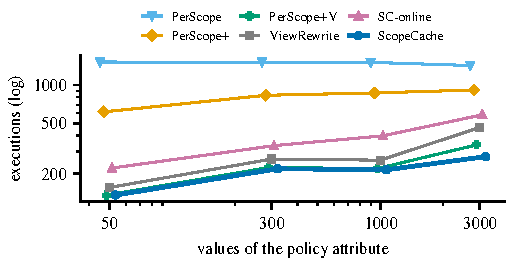
\includegraphics[width=\columnwidth]{fig_domain.pdf}
\caption{\M{SC-hybrid} never needs more executions than the other caches at any domain size, and its lead over the view-based caches grows with the policy domain. Warehouse executions as the policy attribute grows from 50 to 3{,}000 values (development seed 0, about 2{,}400 measured calls per point; lower is better); markers are offset where \M{PerScope+V} and \M{SC-hybrid} coincide.}
\label{fig:domain}
\Description{Warehouse executions of SC-hybrid and the baselines as the policy-attribute domain grows, showing the hybrid never above the other caches and a widening lead over the view-based caches.}
\end{figure}

\textbf{Scale.} At five times the data (TPC-H at scale factor 5, 30 million rows, development seed 0), \M{SC-hybrid} answered all \scaleDataCalls{} data calls without a wrong answer and needed \scaleRedVR\% fewer executions than \M{ViewRewrite} (\scaleRedVROne\% at scale factor 1 with the same seed), \scaleRedPS\% fewer than \M{PerScope}, and \scaleRedPSV\% fewer than \M{PerScope+V}: reuse depends on the workload and the grants, not on the data volume, while each avoided execution grows with it.

\textbf{Overhead.} A hit evaluates the scope on the cells of the candidate entries and merges the selected cells; measured in a separate run of each setup (seed 0) with no other experiment of ours running, it takes \deriveMsLo--\deriveMsHi\,ms on average in our Python implementation, against about 500\,ms for each avoided warehouse call, and the 95th-percentile local time of a call, including executions on a miss, is \lookupPninetyFiveLo--\lookupPninetyFiveHi\,ms. View selection and materialization take at most \viewSelSecMax\,s per run. On the headline grid, holdout selection---paid once, on the training prefix, scoring the five portfolio members---takes \adaptSelSecLo--\adaptSelSecHi\,s of wall time (median \adaptSelSecMed\,s). The ghost directory stores metadata of evicted online entries, not payloads. On the measured suffix, ScopeCache's per-call local latency is indistinguishable from \M{SC-hybrid}'s (median $p_{50}$ \ovhPfiftyOursMed\,ms against \ovhPfiftyHybMed\,ms; range \ovhPfiftyOursLo--\ovhPfiftyOursHi\,ms), and both stay within the $10^6$-row budget. These wall-clock figures are from the same machine as the headline executions and are not mixed with any other server. The scope-keyed path serves distinct counts and entries above the admission bound (\fallbackLo--\fallbackHi\% of data calls) with the same soundness guarantee.

\Takeaway{Cross-scope sharing of partial aggregates, pinned views, and, on the online path, predicate lifting account for the savings; \M{SC-hybrid} keeps its advantage over access-controlled views under interest drift and a ten-times smaller budget, at \deriveMsLo--\deriveMsHi\,ms per hit against about 500\,ms per avoided warehouse call.}

\textbf{Pre-registered robustness.} Table~\ref{tab:rob} evaluates the frozen method on five new unseen seeds (6--10) against every baseline, first under the default Zipf workload and then under a shifted flatter mix (exponents 0.2, 0.2, 0.2) declared before any shifted run. This grid does not replace Table~\ref{tab:main}. On the default workload, ScopeCache matches or beats \M{PerScope+V} in 24 of 25 cells (\robWTLPsv{}; \robRedPsv\% fewer executions in total, \robOurs{} against \robPsv{}; 95\% CI [\robCIpsvLo{}, \robCIpsvHi{}], which excludes zero). The one loss is TPC-H seed 10 (\robLossExec{} executions against \robLossPsv{} for \M{PerScope+V} and \robLossHyb{} for \M{SC-hybrid}): the same validation-horizon unpin as the official TPC-H seed 3 cell---the selector kept the raw-value hybrid, and 42 ghost hits unpinned four views (\lossUnpinRows{} rows)---and on this seed the deficit also trails \M{PerScope+V}. Against \M{SC-hybrid} that grid is \robWTLHyb{} and the 95\% CI ([\robCIhybLo{}, \robCIhybHi{}]) includes zero. On the shifted mix the same method has no losses against either baseline (\shiftWTLPsv{} vs.\ \M{PerScope+V}, \shiftWTLHyb{} vs.\ \M{SC-hybrid}; \shiftRedPsv\% and \shiftRedHyb\% fewer in total; both CIs exclude zero), and TPC-H seed 10 selects $\mathit{pop50}$, does not unpin, and leads both (\shiftTpchTenOurs{} against \shiftTpchTenPsv{} and \shiftTpchTenHyb{}). We do not retune $\mathit{unpin\_min}$ or the portfolio on these seeds.

\begin{table}[t]
\centering
\caption{Pre-registered robustness of the frozen method on unseen seeds 6--10. This evaluation does \emph{not} replace Table~\ref{tab:main} (seeds 3--5: \psvW{}--\psvT{}--\psvL{} vs.\ \M{PerScope+V}). The shifted \texttt{flatmix} (Zipf $0.2,0.2,0.2$) was declared before any shifted run. W--T--L versus each baseline; 95\% CI on the total-execution difference (paired bootstrap, seed \bootSeed{}, \bootB{} replicates). Bold is fewest executions (ScopeCache, in the header); underline is the second-lowest total on that grid.}
\label{tab:rob}
\scriptsize
\setlength{\tabcolsep}{3.0pt}
\begin{tabular}{@{}l cc c cc c@{}}
\toprule
& \multicolumn{3}{c}{Default Zipf (ours \textbf{\robOurs{}})} & \multicolumn{3}{c}{Shifted \texttt{flatmix} (ours \textbf{\shiftOurs{}})}\\
\cmidrule(lr){2-4}\cmidrule(lr){5-7}
vs.\ baseline & W--T--L & Base & 95\% CI & W--T--L & Base & 95\% CI\\
\midrule
\textbf{\M{PerScope+V}} & \textbf{\robWTLPsv{}} & \robPsv{} & [{$-$710}, {$-$171}] & \textbf{\shiftWTLPsv{}} & \shiftPsv{} & [{$-$1576}, {$-$509}]\\
\M{SC-hybrid} & \robWTLHyb{} & \robHyb{} & [{$-$714}, {15}] & \shiftWTLHyb{} & \shiftHyb{} & [{$-$1382}, {$-$385}]\\
\M{SC-online} & 24--0--1 & 11{,}425 & excl.\ 0 & 24--1--0 & 13{,}386 & excl.\ 0\\
\M{SC-atoms} & 6--10--9 & \underline{\robAtoms{}} & [{$-$623}, {8}] & 11--11--3 & \underline{\shiftAtoms{}} & [{$-$1216}, {$-$356}]\\
Others$^{\dagger}$ & 25--0--0 & --- & excl.\ 0 & 25--0--0 & --- & excl.\ 0\\
\bottomrule
\end{tabular}\\[2pt]
{\scriptsize $^{\dagger}$\M{PerScope+}, \M{VR-adapt}, and \M{ViewRewrite}: all 25--0--0 on both grids (CIs exclude zero).}
\end{table}


\textbf{Where ScopeCache wins and where it is second.} ScopeCache saves the most when the holdout reserves budget that a fixed set of views would evict (SYN-FG; TPC-H seeds 4 and 5 on the headline). It is second to \M{SC-hybrid} on TPC-H seed 3 of the headline (348 vs.\ 328, still ahead of \M{PerScope+V} at 352; Table~\ref{tab:main}) and, on the later default-workload grid, on TPC-H seed 10, both from the same validation-horizon unpin (Table~\ref{tab:rob}). An operator who will only deploy the full-view hybrid can run \M{SC-hybrid} and avoid those cells, at the cost of the larger SYN-FG and reserved-budget savings that make the headline 15-cell total, and both 25-cell robustness totals versus \M{PerScope+V}, favor ScopeCache.

\section{Discussion}
\label{sec:discussion}
\textbf{Deployment.} ScopeCache sits below the policy check of a metric tool and above the warehouse, in the trust domain of both, and needs from the platform only the evaluation of a principal's grants as a DNF over policy attributes, the definition hashes of base measures, and the request format of the tool. The metric platform that motivated this work exposes all three: its grants are equality or IN conjunctions per role, combined by union, and every result carries a semantic-snapshot identifier.

\textbf{Generality.} Theorems~\ref{thm:sound}--\ref{thm:republish} hold for distributive aggregates over one fact table between data loads and for policies whose row predicates are DNFs over attributes of that table; these cover the metric layers and grant models above. Policies that refer to other tables (for example, a manager relation) are first resolved to value sets of a policy attribute, as the platforms do when they compile grants. Distinct counts take the scope-keyed path and remain sound; mergeable sketches would let them share across scopes approximately.

\textbf{Storage and confidentiality.} Entries contain aggregates over rows that some requesters may not see, as materialized views and the warehouse's own buffers do. Placing the cache inside the warehouse's trust domain and encrypting it at rest with the warehouse's keys keeps the confidentiality boundary unchanged.

\section{Related Work}
\label{sec:related}

\textbf{Answering queries with views and caches.} Rewriting queries over materialized views~\cite{levy95,halevy01,chaudhuri95,goldstein01}, or predicate and chunk caching~\cite{keller96,deshpande98,kalnis01}, view selection on the cube lattice~\cite{hru96,mistry01}, dynamic and partial materialization~\cite{dynmv07}, and recycling of intermediates~\cite{ivanova09,nagel13,dursun17} reuse work for a single principal. Cloud services reuse common subexpressions~\cite{cloudviews18}, cache results and predicates~\cite{crystal21,predcache24,lbsc24}, and predict views~\cite{mvgpt26}; Snowflake reuses a result only for an identical statement and re-checks the role~\cite{snowflake16}. ScopeCache adds the policy attributes as a grouping dimension of every entry, which makes the derivation rules of view matching safe across principals, and adds the event semantics. BI semantic layers route queries to pre-aggregations declared in the data model~\cite{cubepreagg}; with row-level security, Power BI requires the security expressions to filter both an aggregation table and its detail table~\cite{powerbiagg}, and warehouse row access policies are evaluated at query time~\cite{snowflakerap}. These pre-aggregations are declared offline and refreshed as a whole; ScopeCache creates principal-independent entries online by lifting misses, invalidates only changed measure columns, and proves soundness and non-interference for every derivation. \M{ViewRewrite} models this design.

\textbf{Fine-grained access control.} Query modification~\cite{stonebraker74}, Truman and non-Truman models~\cite{rizvi04}, authorization views~\cite{zhang05}, predicated grants~\cite{chaudhuri07}, disclosure control~\cite{lefevre04}, and provable security definitions~\cite{guarnieri16} define what a principal may see; Kabra et al.\ show how rewriting leaks through side effects~\cite{kabra06}. Sieve scales policy evaluation with guards~\cite{sieve20} and its extension caches guard evaluations~\cite{shakya25}; Data Guard compiles purpose-based policies into masked views~\cite{dataguard26}; HONEYBEE partitions vector indexes along role structure~\cite{honeybee25}. These systems enforce policies per query or cache policy decisions; ScopeCache reuses query results across principals and proves non-interference for them. A concurrent submission by the same authors~\cite{authzgraph26} (AuthZ-Graph, under submission to ICDE~2027) studies a different object: an index that maintains effective permissions over a dynamic authorization graph with conditions and deny, so that a revocation cannot return a stale allow. The present paper does not claim that authorization model or that index; it takes grants, once compiled to a DNF over policy attributes, as given, and studies how a result cache reuses work across the resulting scopes. An earlier draft of this work evaluated a setup derived from the same enterprise authorization source as that submission; that setup has been removed, and every experiment here uses public datasets and fully synthetic policies.

\textbf{Semantic and LLM caches.} OLAP semantic caching canonicalizes queries into intent signatures with roll-up and filter derivation~\cite{bindschaedler26}; GPTCache, MeanCache, and vCache cache LLM responses by similarity, per user, or with error bounds~\cite{gptcache23,meancache24,vcache25}; agentic plan caching reuses plans~\cite{plancache25}. Shared caches leak through timing and key collisions~\cite{gu25,song24,keycoll26}. None of these considers row scopes; ScopeCache provides exact reuse with zero over-privileged answers.

\textbf{Agents over governed data.} Agent-first data systems call for sharing across speculative agent queries~\cite{agentfirst25,wadlom26}; MCP gateways and authorization architectures route agent tool calls through policy engines~\cite{mcpgw26,authzarch26}; recent work defines revocation outcomes and evidence reuse at the gateway~\cite{revocation26,matoi26,notrace26}, studies post-filtering attacks~\cite{plaintext26}, and benchmarks text-to-SQL under access control~\cite{rbact2s26,rolerefusal25}. ScopeCache operates below the gateway, on the results of governed metric tools, and gives a zero staleness window by construction.

\section{Conclusion}
\label{sec:conclusion}

ScopeCache shows that a result cache can serve principals with different row scopes from the same work: entries that group by the policy attributes and contain no principal and no formula admit exact, non-interfering derivation, make permission changes free, and limit republish invalidation to the changed measures. On five setups, including a fine-grained synthetic shop policy, and on traces of real LLM agents over the four public and enterprise-synthetic setups, it returned no wrong answer, and its online path answered \agentXscopeMeanLo--\agentXscopeMeanHi\% of agent data calls from aggregates computed for other scopes. On fifteen runs whose seeds were held out from design and from the choice of the unpinning threshold, it matches or beats the strongest baseline in every run (\psvW{} wins, \psvT{} ties, \psvL{} losses; \freshRedTot\% fewer executions in total) and turns the three SYN-FG losses of the non-adaptive hybrid into wins. Extending the entry format to joins across fact tables and to sketches for distinct counts is future work.

\section*{AI-Generated Content Acknowledgment}
\emph{AI as part of the experimental analysis.} The five LLM agents named in Section~\ref{sec:rq3} (DeepSeek, GLM, Kimi, GPT-6, and Claude Opus~5.5), accessed on the dates and at the settings reported there, generated the recorded tool-call traces; only public and synthetic data were sent to them, and all prompts and responses are released with the artifact.
\emph{Use of AI in preparing this paper.} Claude Opus~5.5 (Anthropic), used through the Claude Code tool, assisted with drafting the text; with the proofs of Lemma~\ref{lem:pure}, Theorems~\ref{thm:sound}--\ref{thm:republish}, and Proposition~\ref{prop:select}; with the implementation and the experiment, analysis, and plotting code; and with bibliographic checks. The authors checked every sentence, derivation, and artifact, additionally validated soundness by the differential test of Section~\ref{sec:rq1}, and take full responsibility for the correctness and originality of the entire content.

\bibliographystyle{ACM-Reference-Format}
\bibliography{references}

\end{document}
